% !TeX root = enterprise-architecture-digital-blueprint.tex
% !TeX encoding = UTF-8
\chapter{Arsitektur Aplikasi dan Teknologi Saat Ini}

\section*{Tujuan Pembelajaran}
\begin{itemize}
  \item Menyusun katalog aplikasi dan menilainya dengan model TIME (\textit{Tolerate, Invest, Migrate, Eliminate}).
  \item Memetakan integrasi antaraplikasi dan menunjukkan titik rawan pola \textit{point-to-point}.
  \item Merangkum lanskap teknologi tingkat tinggi beserta utang teknis dan risikonya.
\end{itemize}

\section{Pendahuluan}

Misalkan pada rapat anggaran 2027 direktur keuangan Medikara mengajukan tiga pertanyaan
singkat: berapa aplikasi yang dimiliki Medikara, berapa biayanya per tahun, dan siapa yang
bertanggung jawab atas tiap aplikasi. Bagian teknologi informasi (TI) menyerahkan daftar
berisi 19 aplikasi. Bagian keuangan menemukan kontrak dan tagihan untuk 18 aplikasi lain.
Para kepala unit masih menyebut 9 aplikasi yang tidak ada di kedua daftar itu. Aplikasi
memang sering bertambah lebih cepat daripada inventarisnya: proyek selesai, kontrak
diperpanjang, dan unit mengembangkan alat sendiri. Tanpa potret yang dapat dipercaya,
keputusan modernisasi mudah mengikuti produk yang paling terlihat.

Medikara memiliki lima versi Sistem Informasi Manajemen Rumah Sakit (SIMRS), aplikasi pasien
Medikara+, dan \textit{Enterprise Resource Planning} (ERP) keuangan terpusat. Integrasi ke
Badan Penyelenggara Jaminan Sosial (BPJS) Kesehatan dan SATUSEHAT berlangsung secara
\textit{point-to-point}, dan banyak laporan manajemen masih disusun dengan
\textit{spreadsheet}. Bab ini memotret kondisi yang berjalan dan menilai alasan mempertahankan
atau mengubahnya. Hasilnya melengkapi Bab 5 dan Bab 6 menjadi dokumen kondisi saat ini untuk
tonggak C2, yang ditinjau menjelang Ujian Tengah Semester (UTS). Keputusan target yang rinci
dilanjutkan pada Bab 9 dan Bab 10.
\IfFileExists{../figures/ch07-diagram-konsep.png}{%
Masalah layanan ditelusuri ke kapabilitas, aplikasi, integrasi, dan
ketergantungan teknologi sebelum arah penanganan portofolio dipilih.
Gambar \ref{fig:ch07-ilustrasi-bab} merangkum hubungan komponen dan konsep utama bab ini.
\begin{figure}[!htb]
  \centering
  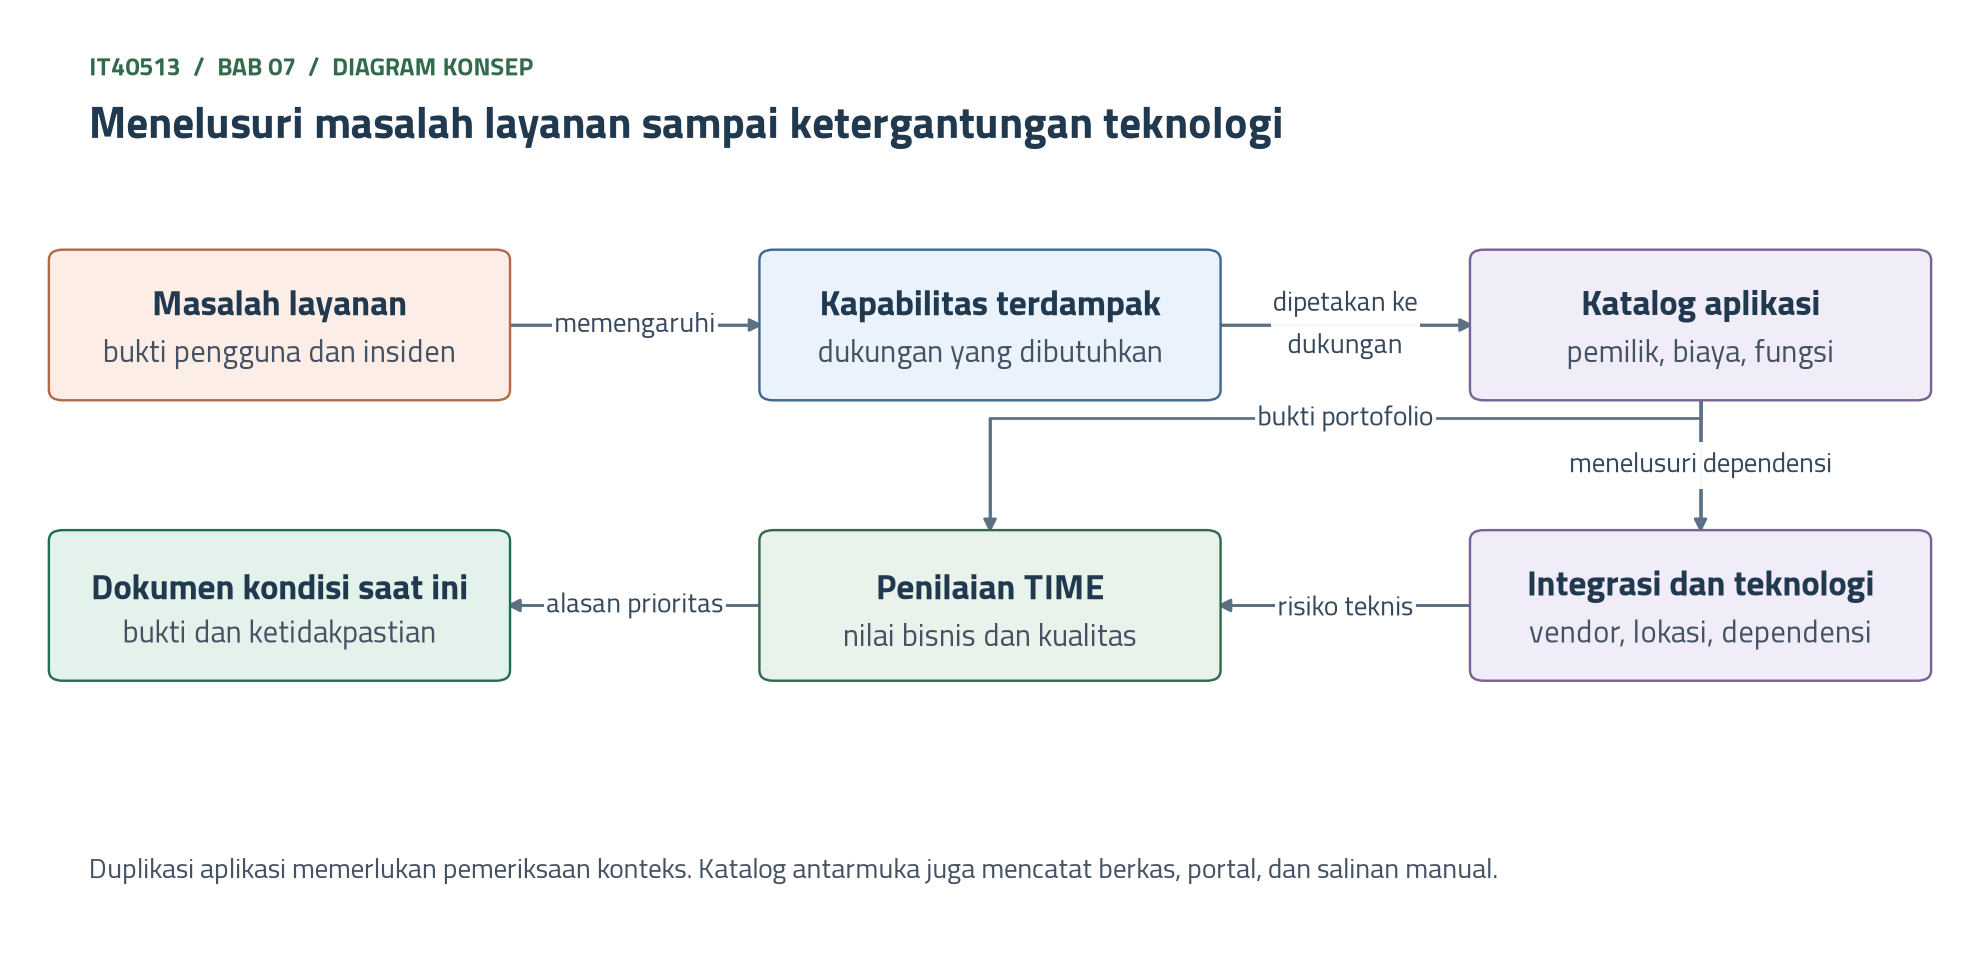
\includegraphics[width=\textwidth]{../figures/ch07-diagram-konsep.png}
  \caption{Menelusuri masalah layanan sampai ketergantungan teknologi}
  \label{fig:ch07-ilustrasi-bab}
\end{figure}
}{}

Bab ini berada pada fase C dan fase D dalam \textit{Architecture Development Method} (ADM)
milik The Open Group Architecture Framework (TOGAF) \cite{togaf10}. Rujukan utama manajemen
portofolio aplikasi adalah Simon, Fischbach, dan Schoder \cite{c07-simon2010}. Model TIME
berasal dari Gartner. Naskah asli Gartner tidak terbuka untuk umum, sehingga bab ini memakai
ringkasan SAP LeanIX \cite{c07-sheppard2023} sebagai sumber sekunder. Gaya integrasi mengikuti
Hohpe dan Woolf \cite{hohpe2003}. Utang teknis mengikuti Cunningham serta Kruchten, Nord,
dan Ozkaya \cite{c07-cunningham1992,c07-kruchten2012}. Pembahasan berjalan dari katalog
aplikasi, pemetaan ke kapabilitas, penilaian TIME, integrasi, lanskap teknologi, utang teknis,
sampai perangkaian dokumen C2.

\section{Katalog Aplikasi}

Katalog aplikasi mencatat sistem yang mendukung pekerjaan organisasi beserta lingkupnya.
Atribut minimumnya meliputi kode, nama, fungsi, pemilik bisnis, pengelola teknis, pengguna,
vendor, versi, umur, lokasi, biaya, serta hubungan dengan data dan layanan. TOGAF menyebut
artefak ini \textit{Application Portfolio Catalog} dan menempatkannya pada fase C
\cite{togaf10}. Simon dan rekan mencatat bahwa banyak organisasi kehilangan jejak lanskap
aplikasinya, sementara kerumitan portofolionya naik tajam. Mereka mengusulkan proses
manajemen portofolio aplikasi dengan empat tahap: pengumpulan data, analisis, pengambilan
keputusan, dan optimasi \cite{c07-simon2010}. Katalog adalah tahap pertama. Tanpa katalog,
tiga tahap berikutnya bekerja dengan angka yang tidak dapat diperiksa.

Analoginya seperti inventaris kendaraan perusahaan. Merek kendaraan saja tidak menunjukkan
siapa memakainya, cabang mana yang menanggung biaya, atau kapan perawatannya berakhir. Lima
kendaraan dengan merek sama tetap memerlukan identitas berbeda jika riwayat dan tanggung
jawabnya berbeda.

Dua contoh dari Medikara Health:

\begin{enumerate}
  \item Misalkan APP-01 sampai APP-05 mewakili instalasi SIMRS di Jakarta, Bekasi, Depok, Bogor,
        dan Bandung. Kontrak vendor tiap instalasi Rp450 juta per tahun, sehingga totalnya
        Rp2,25 miliar. Bila kelimanya ditulis sebagai satu baris ``SIMRS'', perbedaan versi,
        vendor, dan tanggal akhir kontrak hilang dari pandangan direksi.
  \item Misalkan bagian klaim memakai \textit{spreadsheet} dengan makro untuk menggabungkan
        laporan 18 klinik. Berkas itu bukan aplikasi resmi, tetapi 18 klinik bergantung padanya
        setiap bulan. Tim mencatat pemilik, sumber data, pengendalian versi, dan akibat bila
        berkas tidak tersedia. Menyebutnya berkas biasa tidak menghilangkan risikonya.
\end{enumerate}

Sumber inventaris tidak hanya catatan bagian TI. Kontrak, tagihan, daftar akses, wawancara, dan
laporan proses memperlihatkan aplikasi yang tidak terdaftar. Identitas dan fungsi diperoleh dari
daftar aplikasi dan wawancara, tanggung jawab dan biaya dari kontrak dan tagihan, pemakaian dari
daftar akses, dan ketergantungan dari konfigurasi serta peta proses. Tabel
\ref{tab:ch07-rekonsiliasi} memperlihatkan bagaimana katalog awal Medikara berisi 8 aplikasi inti pada Bab 5 tumbuh menjadi
46 aplikasi setelah direkonsiliasi. Bab 9 memakai angka 46 itu sebagai titik awal rasionalisasi.

\begin{table}[!htb]
  \centering
  \caption{Rekonsiliasi katalog aplikasi Medikara (angka pengandaian)}
  \label{tab:ch07-rekonsiliasi}
  \small
  \begin{tabularx}{\textwidth}{>{\raggedright\arraybackslash}p{3.7cm}cc>{\raggedright\arraybackslash}X}
    \hline
    \textbf{Sumber} & \textbf{Tambahan} & \textbf{Jumlah} & \textbf{Contoh yang ditemukan} \\
    \hline
    Katalog awal (Bab 5) & 8 & 8 & Lima SIMRS, SIM Klinik, ERP keuangan, Medikara+ \\
    \hline
    Daftar bagian TI & 11 & 19 & Sistem laboratorium, radiologi, penggajian \\
    \hline
    Kontrak pengadaan & 12 & 31 & Antrean Bandung yang dibeli pada 2021, aplikasi apotek \\
    \hline
    Tagihan unit & 6 & 37 & Langganan \textit{Software as a Service} (SaaS) kecil untuk absensi dan survei pasien \\
    \hline
    Daftar akses dan wawancara & 9 & 46 & Surveilans infeksi Bogor, Laporan Klaim Lama \\
    \hline
  \end{tabularx}
\end{table}

\subsection*{Apa yang dihitung sebagai satu aplikasi?}

Pertanyaan kemudian muncul: apa yang dihitung sebagai satu aplikasi? Tim menyepakati unit
inventaris lebih dahulu, yaitu produk, instalasi, atau layanan. Kelima SIMRS dihitung lima,
karena versi, kontrak, dan lokasinya berbeda, walaupun namanya mirip. SIM Klinik dihitung satu,
karena 18 klinik pratama memakai satu instalasi bersama. \textit{Spreadsheet} laporan dicatat di baris
tersendiri. Bab 9 mencatat 23 berkas di luar hitungan 46 aplikasi, sehingga katalog
Medikara memuat $46 + 23 = 69$ butir yang perlu dinilai. Pilihan unit ini menentukan semua
angka sesudahnya, sehingga ditulis pada halaman pertama katalog.

\subsection*{Siapa pemilik sebuah aplikasi?}

Tiga peran sering tertukar: pemilik bisnis, pengelola teknis, dan vendor. Pembagiannya begini.
Pemilik bisnis bertanggung jawab atas hasil layanan, anggaran, dan kebutuhan perubahan. Pengelola
teknis bertanggung jawab atas pengoperasian, akses, dan koordinasi perubahan. Vendor mengerjakan isi
kontrak, misalnya pengembangan dan dukungan. Pada Medikara+, ketiganya adalah Direktur Pelayanan,
Kepala TI, dan pembuat aplikasi. Vendor dapat menjalankan sistem, tetapi tidak menggantikan tanggung
jawab bisnis organisasi. Satu kolom ``pemilik'' yang mencampur ketiganya menyulitkan keputusan.

\subsection*{Biaya kontrak dan biaya penuh}

Dua hal pada kolom biaya sering tertukar: biaya kontrak dan biaya penuh. Biaya kontrak adalah
angka pada tagihan vendor. Biaya penuh mencakup seluruh ongkos menjalankan aplikasi selama satu
tahun, yang sering disebut \textit{Total Cost of Ownership} (TCO). Tabel
\ref{tab:ch07-biaya-penuh} menguraikannya untuk satu instalasi SIMRS.

\begin{table}[!htb]
  \centering
  \caption{Biaya satu instalasi SIMRS per tahun (angka pengandaian)}
  \label{tab:ch07-biaya-penuh}
  \small
  \begin{tabularx}{\textwidth}{>{\raggedright\arraybackslash}Xr>{\raggedright\arraybackslash}p{4.3cm}}
    \hline
    \textbf{Komponen} & \textbf{Rp juta} & \textbf{Sumber bukti} \\
    \hline
    Kontrak vendor & 450 & Kontrak dan tagihan \\
    \hline
    Lisensi basis data & 280 & Kontrak lisensi \\
    \hline
    Server, sistem operasi, dan ruang server & 190 & Catatan aset dan listrik \\
    \hline
    Staf TI setempat & 220 & Alokasi waktu staf \\
    \hline
    \textbf{Biaya penuh} & \textbf{1.140} & Sekitar 2,5 kali nilai kontrak \\
    \hline
  \end{tabularx}
\end{table}

Pembedaan ini punya dua konsekuensi. Pertama, biaya lima SIMRS bukan Rp2,25 miliar, melainkan
$5 \times \text{Rp1.140 juta} = \text{Rp5,7 miliar}$ per tahun. Bila penawaran SIMRS baru hanya
dibandingkan dengan nilai kontrak, kondisi saat ini tampak Rp3,45 miliar lebih murah daripada
kenyataannya. Kedua, biaya penuh memerlukan alokasi. Staf yang merawat tiga aplikasi harus dibagi
dengan aturan yang tertulis, supaya gajinya tidak terhitung tiga kali.

Setiap nilai memiliki tanggal dan tingkat keyakinan. Biaya yang masih berupa perkiraan ditandai,
dan kontrak yang tidak ditemukan menjadi pekerjaan penelusuran. Katalog bukan kumpulan informasi
yang dianggap pasti hanya karena ditulis dalam tabel. Tim menjaga jejak sumber sehingga pembaca
dapat memeriksa alasan penilaiannya.

\subsection*{Apakah 46 aplikasi terlalu banyak?}

Angka 46 sendiri belum menjawab pertanyaan itu. Mocker meneliti 273 aplikasi di sebuah bank
investasi Eropa dan memisahkan kerumitan arsitektur aplikasi menjadi empat jenis, yaitu yang
berkaitan dengan saling ketergantungan, keragaman, penyimpangan, dan tumpang tindih. Temuannya:
hanya kerumitan saling ketergantungan yang berperilaku seperti asumsi umum, sedangkan jenis lain
menunjukkan efek yang sebagian berlawanan \cite{c07-mocker2009}. Karena itu direksi lebih terbantu
oleh pertanyaan ``aplikasi mana yang saling bergantung, dan apa akibatnya'' daripada oleh jumlah
aplikasi. Pada Medikara, jenis pertama terlihat pada antarmuka, jenis kedua pada empat merek basis
data, dan jenis keempat pada SIM Klinik yang fungsinya mirip modul rawat jalan SIMRS.

\section{Pemetaan Aplikasi ke Kapabilitas}

Matriks aplikasi dan kapabilitas menghubungkan inventaris pada bab ini dengan peta bisnis Bab 5.
Setiap sel menyatakan bentuk dukungan satu aplikasi pada satu kapabilitas. TOGAF menyebut artefak
serupa \textit{Application/Function Matrix} \cite{togaf10}. Banyak aplikasi pada satu kapabilitas
dapat menunjukkan duplikasi, variasi kebutuhan, atau pembagian tugas yang sah. Analisis perlu
mengetahui konteks sebelum menetapkan aplikasi yang akan dihentikan.

Sebaliknya, kapabilitas tanpa aplikasi tidak selalu memerlukan pembelian sistem. Kemampuan
tertentu dapat berjalan baik dengan prosedur dan sarana sederhana. Kesenjangan muncul ketika cara
yang ada gagal memenuhi hasil, volume, risiko, atau waktu yang diperlukan. Bukti \textit{heatmap}
Bab 5 membantu membedakan kebutuhan nyata dari keinginan menambah produk.

Analoginya seperti peralatan dapur katering. Dua alat dapat mengerjakan fungsi yang mirip, tetapi
digunakan di lokasi berbeda atau pada jam yang sama. Menghapus satu alat hanya karena namanya mirip
dapat menurunkan kapasitas. Sebaliknya, membeli alat baru tidak membantu jika masalahnya terletak
pada jadwal kerja dan pembagian tugas.

Dua contoh dari Medikara Health:

\begin{enumerate}
  \item Lima SIMRS dan SIM Klinik sama-sama mendukung Pendaftaran Pasien (CAP-L01), sehingga ada
        enam aplikasi pada satu kapabilitas. Tiap fasilitas memakai definisi pasien lama yang
        berbeda, dan 11,4 persen dari 10.000 nomor rekam medis sampel pada Bab 6 ternyata duplikat
        lintas rumah sakit. Masalah identitas ini tidak selesai hanya dengan menghitung enam
        aplikasi sebagai pemborosan.
  \item Matriks \textit{Create, Read, Update, Delete} (CRUD) Bab 6 mencatat Medikara+ dengan CRUD
        dan SIMRS dengan RU pada konsep Janji Temu. Dua aplikasi menulis data yang sama, padahal
        28 persen kunjungan dipesan lewat Medikara+ dan 72 persen lewat telepon dan loket. Tim
        memeriksa sistem pembuat, sistem pembaca, serta cara rekonsiliasinya.
\end{enumerate}

Tabel \ref{tab:ch07-matriks} memperlihatkan potongan matriks Medikara untuk tujuh kapabilitas.
Kolom SIMRS mewakili lima instalasi. Huruf U berarti dukungan utama, dan huruf P berarti dukungan
pelengkap.

\begin{table}[!htb]
  \centering
  \caption{Potongan matriks aplikasi dan kapabilitas Medikara}
  \label{tab:ch07-matriks}
  \small
  \begin{tabularx}{\textwidth}{>{\raggedright\arraybackslash}Xccccc}
    \hline
    \textbf{Kapabilitas} & \textbf{SIMRS (5)} & \textbf{SIM Klinik} & \textbf{Medikara+} & \textbf{ERP} & \textbf{\textit{Spreadsheet}} \\
    \hline
    L01 Pendaftaran Pasien & U & U & P & & \\
    \hline
    L03 Penjadwalan Layanan & U & U & U & & \\
    \hline
    L04 Pengelolaan Rekam Medis & U & U & P & & \\
    \hline
    P01 Klaim dan Penjaminan & U & P & & P & P \\
    \hline
    P02 Pengelolaan Akses Pengguna & & & & & \\
    \hline
    P03 Pelaporan Manajemen & P & & & P & U \\
    \hline
    P04 Keuangan dan Akuntansi & & & & U & \\
    \hline
  \end{tabularx}
\end{table}

Baris kosong pada P02 layak dibaca dua kali. Misalkan 31 dari 46 aplikasi mengelola akun penggunanya
sendiri. Tidak ada satu aplikasi yang mendukung kapabilitas itu, sehingga temuan audit tentang
kontrol akses yang lemah punya penjelasan arsitektural.

Tiga pola dicari saat membaca matriks. Pola pertama adalah banyak dukungan utama, misalnya L03 dengan
SIMRS, SIM Klinik, dan Medikara+. Pertanyaannya: siapa berwenang mengubah janji temu? Pola kedua adalah
tanpa dukungan utama, misalnya P02. Pertanyaannya: apakah cara yang ada memenuhi kewajiban dan risiko?
Pola ketiga adalah satu aplikasi yang menopang banyak kapabilitas, misalnya SIMRS pada L01, L03, L04, dan
P01. Pertanyaannya: apa saja yang terdampak bila aplikasi berubah?

Pertanyaan kemudian muncul: berapa besar pekerjaan pemetaan ini? Bab 5 menghitung
$15 \times 8 = 120$ sel untuk katalog awal. Dengan 46 aplikasi, ada $15 \times 46 = 690$ sel. Tim
tidak mengisi semuanya sekaligus. Misalkan tim mulai dari 8 aplikasi inti dan 4 kapabilitas merah
pada Bab 5, yaitu L04, P02, P03, dan P06. Ada $8 \times 4 = 32$ sel yang dapat diselesaikan dalam
satu lokakarya. Sel lain diisi bertahap sesuai pertanyaan yang sedang dijawab.

Tim memakai kode kapabilitas dari Bab 5 dan kode konsep informasi dari Bab 6. Jika istilah berubah,
kamus mencatat padanannya. Hubungan tidak dibuat berdasarkan kemiripan nama saja, karena pengguna
perlu mengonfirmasi pekerjaan yang benar-benar didukung aplikasi.

Hasil pemetaan memiliki dua konsekuensi. Pertama, rekomendasi aplikasi dapat ditautkan ke nilai
layanan. Kedua, keputusan penghentian harus menilai seluruh kapabilitas yang bergantung pada aplikasi
itu. Fungsi kecil yang memenuhi kewajiban regulator dapat lebih menentukan daripada fungsi besar yang
mudah diganti.

\section{Penilaian Portofolio dengan Model TIME}

TIME membagi arah penanganan aplikasi menjadi \textit{Tolerate}, \textit{Invest}, \textit{Migrate},
dan \textit{Eliminate}. Dua sumbunya adalah kecocokan fungsi (\textit{functional fit}), yang di modul
ini disebut nilai bisnis, dan kecocokan teknis (\textit{technical fit}), yang di modul ini disebut
kualitas teknis. Menurut ringkasan SAP LeanIX, \textit{Tolerate} berarti menerima aplikasi apa adanya
untuk sementara. \textit{Invest} berarti mengutamakan nilai sebesar-besarnya dari aplikasi prioritas.
\textit{Migrate} berarti mencari aplikasi yang lebih baik untuk kebutuhan yang sama. \textit{Eliminate}
berarti menghapus aplikasi yang tidak lagi diperlukan \cite{c07-sheppard2023}. Riempp dan
Gieffers-Ankel memandang manajemen portofolio aplikasi sebagai sisi arsitektur \textit{enterprise}
yang berorientasi pada keputusan \cite{c07-riempp2007}. TIME melayani tujuan itu: membuka diskusi
keputusan, bukan menggantikannya.

Analoginya seperti menilai bangunan cabang. Gedung yang penting bagi pelanggan tetapi instalasinya
rusak memerlukan perbaikan atau pemindahan, bukan penutupan layanan tanpa pengganti. Gedung yang
jarang dipakai dan rusak mungkin layak dilepas setelah arsip, kontrak, dan penggunanya ditangani.

Dua contoh dari Medikara Health:

\begin{enumerate}
  \item Misalkan SIMRS Bogor memiliki nilai bisnis 5 dan kualitas teknis 2. Arah awalnya
        \textit{Migrate}. Pilihannya dapat berupa peningkatan, penggantian, pemindahan fungsi, atau
        migrasi data. Label tersebut tidak otomatis memerintahkan pindah ke \textit{cloud}.
  \item Misalkan Laporan Klaim Lama memiliki nilai bisnis 2 dan kualitas teknis 2, tetapi masih
        menghasilkan laporan bagi regulator. \textit{Eliminate} tetap bersyarat: fungsi laporan,
        retensi, akses arsip, dan bukti penghentian harus memiliki pengganti yang disetujui.
\end{enumerate}

Gambar \ref{fig:ch07-time} memperlihatkan keempat kuadran, tindakan yang perlu dibuktikan, dan contoh
dari Medikara. Aplikasi juga dapat masuk \textit{Eliminate} bila fungsinya sudah tersedia di aplikasi lain.

\begin{figure}[!htb]
  \centering
  \begin{tikzpicture}[font=\scriptsize,
  sel/.style={draw, text width=4.4cm, minimum height=1.75cm, align=center},
  panah/.style={-{Stealth[length=2mm]}, thick}]
  \node[sel, fill=orange!12] at (0,1.9)
    {\textbf{\textit{Migrate}}\\Nilai tinggi, teknis lemah\\
     {\tiny\mdseries Kemampuan dipertahankan, implementasi diubah}\\
     {\tiny\mdseries Contoh: lima SIMRS}};
  \node[sel, fill=green!10] at (4.8,1.9)
    {\textbf{\textit{Invest}}\\Nilai tinggi, teknis memadai\\
     {\tiny\mdseries Kembangkan dengan ukuran manfaat}\\
     {\tiny\mdseries Contoh: ERP keuangan, Medikara+}};
  \node[sel, fill=red!22] at (0,0)
    {\textbf{\textit{Eliminate}}\\Nilai rendah, teknis lemah\\
     {\tiny\mdseries Penuhi syarat sebelum penghentian}\\
     {\tiny\mdseries Contoh: antrean Bandung, 23 \textit{spreadsheet}}};
  \node[sel, fill=blue!8] at (4.8,0)
    {\textbf{\textit{Tolerate}}\\Nilai rendah, teknis memadai\\
     {\tiny\mdseries Rawat dan tinjau secara berkala}\\
     {\tiny\mdseries Contoh: SIM Klinik}};
  \draw[panah] (-2.55,-1.05)--(7.35,-1.05)
    node[midway, below, font=\tiny] {Kualitas teknis (tinggi bila 4 ke atas, skala 1 sampai 5)};
  \draw[panah] (-2.55,-1.05)--(-2.55,2.95)
    node[midway, above, rotate=90, font=\tiny] {Nilai bisnis (tinggi bila 4 ke atas)};
\end{tikzpicture}

  \caption{Kuadran TIME sebagai bahan keputusan portofolio Medikara}
  \label{fig:ch07-time}
\end{figure}

\subsection*{Indikator dan skala}

Kuadran membantu diskusi, tetapi bukan algoritma keputusan yang lengkap. Skala 1 sampai 5 harus
memiliki indikator. Tabel \ref{tab:ch07-indikator} memuat indikator yang dipakai di kelas. Bobot dan
ambang merupakan pilihan tim yang dicatat, bukan aturan universal TIME. Mata kuliah ini memakai
bobot sama dan menyebut skor 4 ke atas sebagai tinggi.

\begin{table}[!htb]
  \centering
  \caption{Indikator dua sumbu TIME, dengan skor contoh}
  \label{tab:ch07-indikator}
  \small
  \begin{tabularx}{\textwidth}{>{\raggedright\arraybackslash}p{2.4cm}>{\raggedright\arraybackslash}Xcc}
    \hline
    \textbf{Sumbu} & \textbf{Indikator} & \textbf{SIMRS Bogor} & \textbf{Medikara+} \\
    \hline
    Nilai bisnis & Dukungan strategi, kekritisan layanan, cakupan pengguna, kewajiban regulator & 5, 5, 5, 5 & 5, 4, 4, 3 \\
    \hline
    Kualitas teknis & Dukungan vendor dan platform & 2 & 5 \\
    \hline
    Kualitas teknis & Keandalan & 3 & 4 \\
    \hline
    Kualitas teknis & Kemudahan perubahan & 1 & 5 \\
    \hline
    Kualitas teknis & Keamanan dan akses & 2 & 3 \\
    \hline
    Kualitas teknis & Kemudahan integrasi & 2 & 3 \\
    \hline
    \multicolumn{2}{l}{\textbf{Rata-rata nilai bisnis dan kualitas teknis}} & \textbf{5,0 dan 2,0} & \textbf{4,0 dan 4,0} \\
    \hline
  \end{tabularx}
\end{table}

Rata-rata punya kelemahan. Skor Medikara+ pada keamanan dan integrasi hanya 3, tetapi rata-ratanya
tetap 4 karena dukungan dan kemudahan perubahannya tinggi. Kelemahan itu berada pada cara Medikara+
tersambung ke dua SIMRS, bukan pada seluruh aplikasinya, sehingga dicatat di katalog antarmuka.
Aturannya sederhana: setiap indikator penting yang skornya 3 ke bawah dituliskan sebagai syarat
keputusan, walaupun rata-ratanya tinggi.

Tabel \ref{tab:ch07-skor} memuat hasil penilaian aplikasi yang dibahas di bab ini. Arahnya sama
dengan yang dipakai pada tabel rasionalisasi Bab 9.

\begin{table}[!htb]
  \centering
  \caption{Hasil penilaian TIME sebagian aplikasi Medikara (skor pengandaian)}
  \label{tab:ch07-skor}
  \small
  \begin{tabularx}{\textwidth}{>{\raggedright\arraybackslash}p{3.4cm}cc>{\raggedright\arraybackslash}p{1.6cm}>{\raggedright\arraybackslash}X}
    \hline
    \textbf{Aplikasi} & \textbf{Nilai} & \textbf{Teknis} & \textbf{Arah} & \textbf{Syarat atau catatan} \\
    \hline
    Lima SIMRS & 5 & 1 sampai 3 & \textit{Migrate} & Depok paling lemah; layanan dan data aman selama transisi \\
    \hline
    ERP keuangan & 5 & 4 & \textit{Invest} & Sudah terpusat; antarmuka tagihan diperbaiki \\
    \hline
    Medikara+ & 4 & 4 & \textit{Invest} & Akses basis data langsung ditutup lebih dahulu \\
    \hline
    SIM Klinik & 3 & 4 & \textit{Tolerate} & Fungsi mirip modul rawat jalan SIMRS \\
    \hline
    Antrean Bandung & 2 & 2 & \textit{Eliminate} & Fungsi tersedia di Medikara+; data dua tahun dipindahkan \\
    \hline
    Surveilans infeksi Bogor & 2 & 2 & \textit{Eliminate} & Laporan bulanan ke dinas kesehatan harus punya pengganti \\
    \hline
    23 \textit{spreadsheet} laporan & 2 & 1 & \textit{Eliminate} & Laporan wajib dipindah sebelum berkas dihentikan \\
    \hline
  \end{tabularx}
\end{table}

Hasil penilaian ditinjau bersama pemilik bisnis dan pengelola teknis. Perbedaan skor tidak diratakan
tanpa pembahasan. Tim mencatat rentang, bukti, serta alasan keputusan. Kedekatan dengan vendor, umur
aplikasi, atau tampilan antarmuka tidak cukup untuk menetapkan nilai bisnis maupun kualitas teknisnya.

\begin{kasus}[title={Kasus Medikara Health: Sebaran 46 Aplikasi dan Biayanya}]
  Misalkan seluruh katalog sudah dinilai. Tabel \ref{tab:ch07-sebaran} memuat sebarannya. Biaya yang
  dipakai adalah biaya penuh per tahun, totalnya Rp12,2 miliar.

  \begin{center}
    \captionof{table}{Sebaran portofolio aplikasi Medikara menurut arah TIME (angka pengandaian)}
    \label{tab:ch07-sebaran}
    \small
    \begin{tabularx}{\linewidth}{>{\raggedright\arraybackslash}p{1.7cm}crc>{\raggedright\arraybackslash}X}
      \hline
      \textbf{Arah} & \textbf{Jumlah} & \textbf{Rp juta} & \textbf{Porsi} & \textbf{Isi utama} \\
      \hline
      \textit{Invest} & 9 & 2.900 & 23,8\% & ERP keuangan, Medikara+ \\
      \hline
      \textit{Migrate} & 11 & 6.860 & 56,2\% & Lima SIMRS (Rp5.700 juta) \\
      \hline
      \textit{Tolerate} & 14 & 1.520 & 12,5\% & SIM Klinik \\
      \hline
      \textit{Eliminate} & 12 & 920 & 7,5\% & Antrean Bandung, surveilans Bogor \\
      \hline
      \textbf{Jumlah} & \textbf{46} & \textbf{12.200} & \textbf{100\%} & \\
      \hline
    \end{tabularx}
  \end{center}

  Tabel itu mematahkan satu dugaan awal direksi, yaitu bahwa penghematan terbesar datang dari menghapus
  aplikasi. Kelompok \textit{Eliminate} berisi 12 aplikasi, atau 26,1 persen dari jumlah aplikasi,
  tetapi hanya menyerap 7,5 persen biaya. Bila seluruhnya dihentikan, penghematan kotornya paling
  banyak Rp920 juta per tahun. Sebaliknya, 11 aplikasi \textit{Migrate} menyerap 56,2 persen biaya, dan
  lima SIMRS saja menyerap 46,7 persen. Keputusan yang paling berpengaruh ada pada cara menangani
  SIMRS. Penggantiannya tetap menunggu analisis data pasien, antarmuka, kemampuan vendor, serta biaya
  dan risiko transisi.
\end{kasus}

\subsection*{Dua hal yang sering tertukar}

Dua hal pada TIME sering tertukar. Pembagiannya begini. Pertama, \textit{Migrate} pada TIME berbeda
dari pindah ke \textit{cloud}. TIME menjelaskan arah portofolio. Pilihan teknis kemudian dianalisis
bersama arsitektur target dan mata kuliah IT40713. Aplikasi bernilai tinggi dapat dimodernisasi tanpa
mengubah lokasi infrastrukturnya. Kedua, TIME berbeda dari rasionalisasi pada Bab 9. TIME menilai
kondisi aplikasi saat ini. Rasionalisasi memutuskan nasib aplikasi di kondisi target, dengan
pertimbangan kapabilitas target, prinsip arsitektur, dan aplikasi lain yang fungsinya sama.

\section{Integrasi dan Antarmuka}

Katalog antarmuka menyebut sistem pengirim dan penerima, tujuan pertukaran, jenis data, frekuensi,
pola, pemilik, serta penanganan kegagalan. TOGAF menyebutnya \textit{Interface Catalog} dan
menempatkannya pada fase C. Tujuannya menentukan lingkup ketergantungan antaraplikasi sedini mungkin
\cite{togaf10}. Antarmuka dapat berupa layanan otomatis, pertukaran berkas, unggah portal, atau salinan
manual. Peta yang hanya menampilkan \textit{Application Programming Interface} (API) resmi akan melewatkan
aliran \textit{spreadsheet} yang mungkin menentukan laporan dan layanan.

Pola \textit{point-to-point} menghubungkan pasangan sistem secara langsung, tanpa perantara bersama. Pola
ini dapat memadai untuk sedikit hubungan yang stabil. Perubahan menjadi sulit ketika setiap pasangan
memiliki format dan aturan berbeda. Pola perlu dinilai menurut hubungan yang benar-benar ada, frekuensi
perubahan, dan dampak kegagalan.

Analoginya seperti jadwal pengiriman antarcabang. Beberapa rute langsung dapat efisien. Jika setiap
cabang membuat kesepakatan berbeda dengan semua cabang lain, perubahan alamat atau aturan paket memerlukan
banyak penyesuaian. Masalahnya bukan sekadar banyaknya garis, melainkan aturan serta tanggung jawab pada
tiap hubungan.

Dua contoh dari Medikara Health:

\begin{enumerate}
  \item Sembilan sistem terdiri dari lima SIMRS, ERP, Medikara+, BPJS Kesehatan, dan SATUSEHAT. Jika setiap
        pasangan memiliki satu hubungan, batas kombinatorialnya adalah $9 \times 8 / 2 = 36$ pasangan. Itu
        batas atas model sederhana, bukan jumlah antarmuka Medikara yang sudah diamati.
  \item Bab 1 mencatat bahwa perubahan aturan klaim BPJS Kesehatan dikerjakan lima kali, sekali untuk tiap
        SIMRS. Misalkan ada 7 perubahan aturan per tahun, dan tiap pengerjaan butuh 40 jam kerja. Maka ada
        $7 \times 5 = 35$ permintaan perubahan dan $35 \times 40 = 1.400$ jam kerja per tahun. Bukti
        semacam ini lebih berguna bagi direksi daripada pernyataan bahwa seluruh integrasi harus diganti.
\end{enumerate}

Tiap antarmuka dinilai dengan tiga pertanyaan risiko. Untuk tujuan dan data: apakah data minimum dan dasar
aksesnya jelas? Untuk operasi: apa yang terjadi saat koneksi gagal? Untuk tanggung jawab: siapa menguji serta
menyelesaikan selisih?

\subsection*{Empat gaya integrasi}

Pertanyaan kemudian muncul: bagaimana dua aplikasi bertukar data? Hohpe dan Woolf menyebut empat gaya:
transfer berkas, basis data bersama, panggilan prosedur jarak jauh, dan pesan \cite{hohpe2003}. Tabel
\ref{tab:ch07-gaya} menjelaskan keempatnya dan menghitung pemakaiannya pada katalog Medikara. Kolom gaya
perlu diisi, karena gaya menentukan risikonya. Dua antarmuka yang menyambungkan pasangan aplikasi yang
sama dapat punya risiko yang jauh berbeda.

\begin{table}[!htb]
  \centering
  \caption{Empat gaya integrasi dan pemakaiannya pada katalog Medikara (angka pengandaian)}
  \label{tab:ch07-gaya}
  \small
  \begin{tabularx}{\textwidth}{>{\raggedright\arraybackslash}p{2.5cm}>{\raggedright\arraybackslash}Xc>{\raggedright\arraybackslash}p{3.2cm}}
    \hline
    \textbf{Gaya} & \textbf{Cara kerja} & \textbf{Jumlah} & \textbf{Contoh} \\
    \hline
    Transfer berkas & Satu aplikasi membuat berkas yang dibaca aplikasi lain & 11 & Klaim ke BPJS Kesehatan, tagihan ke ERP \\
    \hline
    Basis data bersama & Aplikasi berbagi satu basis data & 2 & Medikara+ ke SIMRS Bekasi dan Bogor \\
    \hline
    Panggilan prosedur jarak jauh & Aplikasi membuka prosedur yang dipanggil aplikasi lain, disebut panggilan layanan pada katalog & 13 & Eligibilitas BPJS Kesehatan, SATUSEHAT \\
    \hline
    Pesan & Aplikasi bertukar pesan lewat sistem pesan bersama & 0 & Belum ada \\
    \hline
    \textbf{Jumlah otomatis} & & \textbf{26} & \\
    \hline
  \end{tabularx}
\end{table}

\subsection*{Berapa koneksi yang mungkin dan berapa yang ada?}

Rumus $n(n-1)/2$ menghitung pasangan tak berarah pada graf lengkap sederhana. Untuk 9 sistem hasilnya 36.
Bila arah dihitung terpisah, batasnya $n(n-1) = 72$. Setiap sistem baru menambah koneksi sebanyak jumlah
sistem yang sudah ada. Misalkan tiga mitra ditambahkan, sehingga ada 12 sistem. Batasnya naik dari 36 menjadi
$12 \times 11 / 2 = 66$ pasangan. Inilah alasan strategi ekosistem mitra pada 2026 sampai 2030 tidak dapat
berjalan di atas pola ini. Perbandingannya dengan \textit{hub} dibahas pada Bab 9.

Batas itu belum menjawab berapa koneksi yang sungguh ada. Bab 1 mencatat 20 sambungan dari lima SIMRS ke
empat sistem lain. Misalkan katalog menambah satu pasangan Medikara+ dengan ERP untuk pembayaran telekonsultasi,
sehingga ada 21 pasangan aktif. Gambar \ref{fig:ch07-matriks-pasangan} memperlihatkan semua 36 pasangan itu.
Angka pada tiap sel memperlihatkan bahwa pasangan dan antarmuka berbeda: pasangan SIMRS dengan BPJS Kesehatan
memuat dua antarmuka, yaitu eligibilitas dan klaim, sehingga 21 pasangan memuat 26 antarmuka otomatis. Sembilan
sistem ini adalah lingkup latihan. SIM Klinik dan 38 aplikasi lain juga punya antarmuka, dan katalog tim harus
memuatnya.

\begin{figure}[!htb]
  \centering
  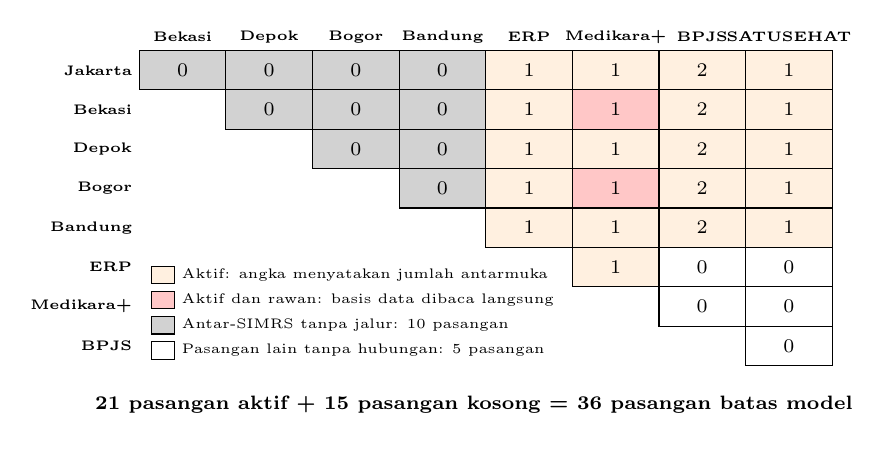
\begin{tikzpicture}[font=\scriptsize,
  sel/.style={draw, minimum width=1.1cm, minimum height=0.5cm, inner sep=0pt},
  aktif/.style={sel, fill=orange!12},
  rawan/.style={sel, fill=red!22},
  hampa/.style={sel, fill=gray!35},
  nol/.style={sel, fill=white},
  kepala/.style={font=\tiny\bfseries, inner sep=1pt},
  tanda/.style={draw, minimum width=0.3cm, minimum height=0.22cm, inner sep=0pt},
  ket/.style={font=\tiny, anchor=west, inner sep=1pt}]
  \foreach \kolom/\nama in {2/Bekasi, 3/Depok, 4/Bogor, 5/Bandung, 6/ERP,
      7/Medikara+, 8/BPJS, 9/SATUSEHAT} {
    \node[kepala] at (\kolom*1.1,0.42) {\nama};
  }
  \foreach \baris/\nama in {1/Jakarta, 2/Bekasi, 3/Depok, 4/Bogor, 5/Bandung,
      6/ERP, 7/Medikara+, 8/BPJS} {
    \node[kepala, anchor=east] at (1.6,-\baris*0.5+0.5) {\nama};
  }
  \foreach \baris/\kolom in {1/2, 1/3, 1/4, 1/5, 2/3, 2/4, 2/5, 3/4, 3/5, 4/5} {
    \node[hampa] at (\kolom*1.1,-\baris*0.5+0.5) {0};
  }
  \foreach \baris in {1,...,5} {
    \node[aktif] at (6*1.1,-\baris*0.5+0.5) {1};
    \node[aktif] at (8*1.1,-\baris*0.5+0.5) {2};
    \node[aktif] at (9*1.1,-\baris*0.5+0.5) {1};
  }
  \foreach \baris in {1,3,5} {
    \node[aktif] at (7*1.1,-\baris*0.5+0.5) {1};
  }
  \foreach \baris in {2,4} {
    \node[rawan] at (7*1.1,-\baris*0.5+0.5) {1};
  }
  \node[aktif] at (7*1.1,-6*0.5+0.5) {1};
  \foreach \baris/\kolom in {6/8, 6/9, 7/8, 7/9, 8/9} {
    \node[nol] at (\kolom*1.1,-\baris*0.5+0.5) {0};
  }
  \node[tanda, fill=orange!12] at (1.95,-2.6) {};
  \node[ket] at (2.15,-2.6) {Aktif: angka menyatakan jumlah antarmuka};
  \node[tanda, fill=red!22] at (1.95,-2.92) {};
  \node[ket] at (2.15,-2.92) {Aktif dan rawan: basis data dibaca langsung};
  \node[tanda, fill=gray!35] at (1.95,-3.24) {};
  \node[ket] at (2.15,-3.24) {Antar-SIMRS tanpa jalur: 10 pasangan};
  \node[tanda, fill=white] at (1.95,-3.56) {};
  \node[ket] at (2.15,-3.56) {Pasangan lain tanpa hubungan: 5 pasangan};
  \node[font=\scriptsize\bfseries] at (5.9,-4.25)
    {21 pasangan aktif + 15 pasangan kosong = 36 pasangan batas model};
\end{tikzpicture}

  \caption{Matriks 36 pasangan pada sembilan sistem Medikara, dengan jumlah antarmuka per pasangan}
  \label{fig:ch07-matriks-pasangan}
\end{figure}

Matriks itu juga memperlihatkan hal yang tidak terlihat pada daftar. Sepuluh pasangan antar-SIMRS kosong, karena
kelima SIMRS tidak saling terhubung. Inilah sebabnya riwayat alergi yang tercatat di Bekasi tidak terbaca oleh
dokter di Depok. Masalah terbesar pada pola ini bukan hanya sambungan yang terlalu banyak, tetapi juga sambungan
yang dibutuhkan namun tidak pernah ada.

Gambar \ref{fig:ch07-integrasi-saat-ini} memperlihatkan pandangan yang sama per kelompok, ditambah aliran manual
yang tidak tercatat pada diagram integrasi mana pun menurut Bab 6. Dengan tujuh ekspor manual itu, katalog
Medikara memuat $26 + 7 = 33$ antarmuka.

\begin{figure}[!htb]
  \centering
  \begin{tikzpicture}[font=\scriptsize,
  sistem/.style={draw, rounded corners, text width=2.1cm, minimum height=0.62cm,
    align=flush center, fill=blue!8},
  luar/.style={sistem, fill=orange!12},
  rs/.style={draw, rounded corners, text width=1.8cm, minimum height=0.44cm,
    align=flush center, fill=blue!8, font=\tiny, inner sep=1pt},
  panah/.style={-{Stealth[length=2mm]}, thick},
  duaarah/.style={{Stealth[length=2mm]}-{Stealth[length=2mm]}, thick},
  manual/.style={panah, dashed, red!70!black},
  ket/.style={font=\tiny, inner sep=1.5pt}]
  \draw[rounded corners, fill=praditagreen!15] (0,2.35) rectangle (2.5,-1.85);
  \node[font=\scriptsize\bfseries] at (1.25,2.05) {Lima SIMRS};
  \node[rs] at (1.25,1.6) {Jakarta};
  \node[rs] at (1.25,1.0) {Bekasi};
  \node[rs] at (1.25,0.4) {Depok};
  \node[rs] at (1.25,-0.2) {Bogor};
  \node[rs] at (1.25,-0.8) {Bandung};
  \node[font=\tiny, align=flush center] at (1.25,-1.42)
    {\textit{on-premise},\\versi berbeda};

  \node[luar] (bpjs) at (9.2,1.75) {BPJS Kesehatan};
  \node[luar] (ss) at (9.2,0.65) {SATUSEHAT};
  \node[sistem] (erp) at (9.2,-0.45) {ERP keuangan};
  \node[sistem] (plus) at (9.2,-1.55) {Medikara+};

  \draw[duaarah] (2.5,1.75)--(bpjs.west)
    node[midway, above, ket] {5 pasangan, 10 antarmuka: eligibilitas dan klaim};
  \draw[panah] (2.5,0.65)--(ss.west)
    node[midway, above, ket] {5 pasangan, 5 antarmuka: rata-rata terkirim 3 hari};
  \draw[panah] (2.5,-0.45)--(erp.west)
    node[midway, above, ket] {5 pasangan, 5 antarmuka: tagihan};
  \draw[duaarah, draw=red!70!black] (2.5,-1.55)--(plus.west)
    node[midway, above, ket, text=red!70!black]
      {5 pasangan, 5 antarmuka: 2 membaca basis data langsung};
  \draw[panah] (plus.north)--(erp.south)
    node[midway, right, ket] {1 pasangan};

  \node[draw, rounded corners, fill=green!10, text width=2.1cm, align=flush center,
    minimum height=0.7cm] (laporan) at (1.25,-3.0)
    {Laporan direksi\\{\tiny\mdseries terbit hari kerja ke-12}};
  \node[draw, dashed, rounded corners, fill=red!22, text width=2.7cm, align=flush center,
    minimum height=0.7cm] (spread) at (5.0,-3.0)
    {23 \mbox{\textit{spreadsheet}} laporan\\{\tiny\mdseries 144 hari-orang per tahun}};
  \draw[manual] (2.1,-1.85)--(spread.north west)
    node[midway, right=2pt, ket] {5 ekspor manual};
  \draw[manual] (spread.west)--(laporan.east);
  \draw[manual] (erp.east)--++(0.35,0)|-(spread.east);
  \draw[manual] (plus.south)|-(spread.east);
  \node[ket] at (8.3,-3.2) {2 ekspor manual: ERP dan Medikara+};
  \node[font=\tiny, text width=10.6cm, align=flush center] at (5.2,-4.0)
    {Garis utuh: antarmuka otomatis. Garis putus merah: aliran manual. Jingga: sistem
     eksternal. Angka antarmuka adalah pengandaian pembelajaran.};
\end{tikzpicture}

  \caption{Integrasi Medikara saat ini per kelompok, termasuk aliran manual ke laporan direksi}
  \label{fig:ch07-integrasi-saat-ini}
\end{figure}

\subsection*{Titik rawan pola point-to-point}

Tabel \ref{tab:ch07-titik-rawan} merangkum lima titik rawan yang terbaca dari katalog. Tiap titik rawan punya
bukti, sehingga dapat diperiksa ulang.

\begin{table}[!htb]
  \centering
  \caption{Titik rawan integrasi Medikara}
  \label{tab:ch07-titik-rawan}
  \small
  \begin{tabularx}{\textwidth}{>{\raggedright\arraybackslash}p{3.0cm}>{\raggedright\arraybackslash}X>{\raggedright\arraybackslash}X}
    \hline
    \textbf{Titik rawan} & \textbf{Bukti} & \textbf{Akibat} \\
    \hline
    Perubahan berulang & Satu aturan klaim dikerjakan lima kali & Biaya dan peluang salah berlipat \\
    \hline
    Akses langsung ke basis data & Dua pasangan memakai satu akun bersama (Bab 9) & Paparan data tidak terbatas pada data yang perlu \\
    \hline
    Keterlambatan tanpa pemantauan & Data ke SATUSEHAT rata-rata 3 hari (Bab 6) & Kegagalan baru diketahui belakangan \\
    \hline
    Jalur manual & Tujuh ekspor, 144 hari-orang per tahun (Bab 6) & Tanpa kontrol akses dan riwayat perubahan \\
    \hline
    Jalur yang tidak ada & Sepuluh pasangan antar-SIMRS kosong & Riwayat pasien tidak ikut pindah \\
    \hline
  \end{tabularx}
\end{table}

BPJS Kesehatan dan SATUSEHAT merupakan sistem eksternal. Tim tidak menilai kualitas internalnya berdasarkan dugaan.
Katalog mencatat kemampuan dan kendala integrasi yang dapat dibuktikan dari sisi Medikara. Dari sisi arsitektur, ada
dua hal yang perlu dicatat. Pertama, kewajibannya datang dari luar. Kementerian Kesehatan menyatakan fasilitas
pelayanan kesehatan wajib menerapkan rekam medis elektronik paling lambat 31 Desember 2023, dan SATUSEHAT
mengintegrasikan data kesehatan individu antarfasilitas \cite{c07-kemenkes2023rme}. Kedua, jadwal perubahan juga datang
dari luar. Panduan implementasi SATUSEHAT berbasis \textit{Health Level Seven Fast Healthcare Interoperability
Resources} (HL7 FHIR) R4 dan statusnya masih rilis pendahuluan \cite{c07-satusehat-ig}, sehingga Medikara perlu siap
menghadapi perubahan yang tidak ditentukannya sendiri. Desain kontrak serta keamanan API dibahas rinci pada IT40613.
Penilaian risiko organisasi dibahas pada IT40813.

\begin{kasus}[title={Kasus Medikara Health: Menjawab Pertanyaan Direktur Keuangan}]
  Bab 2 mencatat pertanyaan direktur keuangan: berapa biaya integrasi per tahun, dan integrasi mana yang paling mahal?
  Bab 3 mencatat bahwa Medikara belum pernah mencatat biaya integrasinya per antarmuka, sementara presentasi vendor
  menjanjikan penghematan 30 persen. Misalkan katalog antarmuka kini dilengkapi data insiden dan permintaan perubahan
  satu tahun. Tabel \ref{tab:ch07-biaya-integrasi} memuat hasilnya.

  \begin{center}
    \captionof{table}{Biaya integrasi Medikara per kelompok, per tahun (angka pengandaian)}
    \label{tab:ch07-biaya-integrasi}
    \small
    \begin{tabularx}{\linewidth}{>{\raggedright\arraybackslash}Xccccr}
      \hline
      \textbf{Kelompok} & \textbf{Pasangan} & \textbf{Antarmuka} & \textbf{Insiden} & \textbf{Perubahan} & \textbf{Rp juta} \\
      \hline
      SIMRS dan BPJS Kesehatan & 5 & 10 & 20 & 35 & 480 \\
      \hline
      SIMRS ke SATUSEHAT & 5 & 5 & 45 & 21 & 390 \\
      \hline
      Medikara+ dan SIMRS & 5 & 5 & 40 & 20 & 370 \\
      \hline
      SIMRS ke ERP & 5 & 5 & 20 & 8 & 210 \\
      \hline
      Medikara+ ke ERP & 1 & 1 & 1 & 0 & 20 \\
      \hline
      \textbf{Jumlah} & \textbf{21} & \textbf{26} & \textbf{126} & \textbf{84} & \textbf{1.470} \\
      \hline
    \end{tabularx}
  \end{center}

  Biaya tiap kelompok berasal dari tiga komponen: tenaga menangani insiden, tenaga mengerjakan perubahan, dan operasi
  rutin per pasangan. Cara menghitungnya ada pada kotak pendalaman di seksi Aktivitas. Jawaban untuk direktur keuangan
  kini punya angka: Rp1.470 juta per tahun, rata-rata Rp70 juta per pasangan aktif, dan kelompok BPJS Kesehatan paling
  mahal dengan porsi 32,7 persen. Baris Medikara+ dan SIMRS adalah lima integrasi yang terlihat pada \textit{view} tim TI di
  Bab 4. Janji vendor juga dapat diuji. Penghematan 30 persen berarti Rp441 juta per tahun, dan tim dapat bertanya komponen
  mana yang akan turun. Aliran manual sebesar 144 hari-orang berada di luar angka ini.
\end{kasus}

\begin{pendalaman}[title={Pendalaman Teknis (opsional): Dua Arti Point-to-Point}]
  Istilah \textit{point-to-point} punya dua arti yang berbeda. Pada bab ini, istilah itu menyatakan pola arsitektur:
  pasangan aplikasi tersambung langsung, masing-masing dengan format dan aturan sendiri. Dalam katalog pola Hohpe dan
  Woolf, \textit{Point-to-Point Channel} adalah kanal pada sistem pesan yang menjamin satu pesan diterima oleh satu
  penerima saja \cite{hohpe2003}. Kanal itu dapat berjalan di atas perantara pesan bersama, sehingga pola
  arsitekturnya justru bukan \textit{point-to-point} dalam arti bab ini. Saat membaca dokumen vendor, tim perlu
  memeriksa arti mana yang dimaksud.
\end{pendalaman}

\section{Lanskap Teknologi Tingkat Tinggi}

Lanskap teknologi merangkum lokasi penerapan, \textit{hosting}, platform, jaringan, ketergantungan, dukungan vendor, serta
mekanisme pemulihan yang relevan bagi arsitektur. TOGAF menempatkan \textit{Technology Portfolio Catalog} pada fase D
\cite{togaf10}. Tim tidak perlu menyalin semua alamat perangkat. Informasi yang dipilih harus membantu menjelaskan batas
perubahan, risiko, kapasitas, dan biaya layanan.

Analoginya seperti denah evakuasi gedung. Denah itu tidak memuat setiap kabel dan pipa. Isinya tangga darurat, hidran,
titik kumpul, dan jalur yang harus tetap terbuka. Rinciannya cukup untuk mengambil keputusan saat gedung bermasalah,
dan rincian lain disimpan di dokumen teknis.

Dua contoh dari Medikara Health:

\begin{enumerate}
  \item Bab 10 mencatat dua klinik di pinggiran Bogor yang hanya punya satu jalur internet. Misalkan jalur itu putus dua kali
        dalam satu bulan, masing-masing tiga jam. Pendaftaran di kedua klinik berhenti selama total 6 jam untuk tiap klinik.
        Gangguan ini tidak dijawab dengan membeli server baru, karena sumber masalahnya ada pada konektivitas.
  \item Bab 10 mencatat empat merek basis data pada katalog teknologi Medikara, dengan lisensi dan dukungan Rp2,4 miliar per
        tahun. Dengan dua administrator per merek agar ada pengganti saat cuti, ada delapan orang yang harus disiapkan. Angka
        ini lebih berguna bagi direksi daripada daftar nama produknya.
\end{enumerate}

Gambar \ref{fig:ch07-lanskap-teknologi} merangkum lanskap teknologi Medikara per lokasi. Rinciannya pengandaian yang mengikuti
fakta pada Bab 9 dan Bab 10. Kolom pertama sampai ketiga memperlihatkan \textit{hosting} sendiri, sedangkan kolom keempat
memperlihatkan \textit{hosting} oleh vendor. Baris terbawah adalah temuan yang perlu masuk ke dokumen C2.

\begin{figure}[!htb]
  \centering
  \begin{tikzpicture}[font=\tiny,
  kepala/.style={draw, fill=praditagreen!15, text width=2.36cm, minimum height=0.6cm,
    align=flush center, font=\tiny\bfseries, inner sep=2pt},
  isi/.style={draw, fill=blue!8, text width=2.36cm, minimum height=0.84cm,
    align=flush center, inner sep=2pt},
  rawan/.style={isi, fill=red!22},
  baris/.style={font=\tiny\bfseries, text width=1.05cm, align=flush right, inner sep=1pt}]
  \node[kepala] at (2.0,0) {Ruang server RS Jakarta};
  \node[kepala] at (4.65,0) {Empat ruang server rumah sakit lain};
  \node[kepala] at (7.3,0) {Klinik, laboratorium, dan apotek};
  \node[kepala] at (9.95,0) {Lingkungan vendor};

  \node[baris] at (0.0,-0.82) {Aplikasi};
  \node[isi] at (2.0,-0.82) {SIMRS Jakarta, ERP keuangan, SIM Klinik};
  \node[isi] at (4.65,-0.82) {SIMRS Bekasi, Depok, Bogor, Bandung};
  \node[isi] at (7.3,-0.82) {Pemakai SIM Klinik, aplikasi laboratorium dan apotek};
  \node[isi] at (9.95,-0.82) {Medikara+, catatan telekonsultasi};

  \node[baris] at (0.0,-1.74) {Platform};
  \node[isi] at (2.0,-1.74) {Server fisik, basis data komersial};
  \node[isi] at (4.65,-1.74) {Server fisik, versi berbeda per lokasi};
  \node[isi] at (7.3,-1.74) {Komputer pemakai, sedikit server lokal};
  \node[isi] at (9.95,-1.74) {Dikelola vendor};

  \node[baris] at (0.0,-2.66) {Jaringan};
  \node[isi, text width=5.01cm] at (3.325,-2.66)
    {Jaringan sewaan antar-rumah sakit};
  \node[isi] at (7.3,-2.66) {Internet, sebagian klinik satu jalur};
  \node[isi] at (9.95,-2.66) {Internet ke API bawaan dua SIMRS};

  \node[baris] at (0.0,-3.58) {Temuan};
  \node[rawan] at (2.0,-3.58) {Tanpa lokasi cadangan};
  \node[rawan] at (4.65,-3.58) {Sistem operasi lama, dukungan berbeda};
  \node[rawan] at (7.3,-3.58) {Dua klinik Bogor berhenti bila jalur putus};
  \node[rawan] at (9.95,-3.58) {Akun bersama, data uji tidak disamarkan};

  \node[draw, fill=green!10, text width=10.51cm, minimum height=0.56cm, align=flush center,
    inner sep=2pt] at (5.975,-4.42)
    {Katalog teknologi: 4 merek basis data, 3 keluarga sistem operasi server, 2 alat
     cadangan, 6 alat pelaporan};
\end{tikzpicture}

  \caption{Lanskap teknologi Medikara per lokasi, dengan temuan yang perlu ditindaklanjuti}
  \label{fig:ch07-lanskap-teknologi}
\end{figure}

Tiap aspek punya bukti dan implikasinya. Lokasi dan \textit{hosting} menentukan batas penempatan dan kewajiban data.
Versi, tanggal dukungan, dan kontrak menentukan pilihan perubahan dan tenggatnya. Ketergantungan jaringan dan jalur
cadangan menentukan ketersediaan layanan. Cadangan serta hasil uji pemulihan menentukan kemampuan memenuhi target
layanan.

Pemulihan layak diperiksa pada kondisi saat ini, bukan hanya pada kondisi target. Bab 10 mengutip Permenkes 24/2022 yang mewajibkan
cadangan rekam medis elektronik diletakkan di tempat yang berbeda dari lokasi fasilitas \cite{permenkes24-2022}. Ruang server RS Jakarta
belum punya lokasi cadangan, dan tim mencatatnya sebagai temuan.

\subsection*{Dukungan aplikasi dan dukungan platform}

Dua hal pada kolom dukungan sering tertukar: dukungan aplikasi oleh vendor dan dukungan platform di bawahnya. Pembagiannya begini.
Bab 12 mengandaikan vendor SIMRS lama masih mendukung aplikasinya sampai akhir 2030. Janji itu belum berarti sistem operasi dan basis
data di bawahnya masih menerima pembaruan keamanan. Misalkan SIMRS Depok, yang versinya paling tua, berjalan di atas dua produk pada Tabel
\ref{tab:ch07-siklus-hidup}. Keduanya hanya contoh publik untuk latihan membaca halaman siklus hidup, bukan inventaris faktual Medikara.

\begin{table}[!htb]
  \centering
  \caption{Contoh pembacaan siklus hidup produk, diperiksa 30 Oktober 2026}
  \label{tab:ch07-siklus-hidup}
  \small
  \begin{tabularx}{\textwidth}{>{\raggedright\arraybackslash}Xcc>{\raggedright\arraybackslash}p{3.8cm}}
    \hline
    \textbf{Produk} & \textbf{Dukungan berakhir} & \textbf{Program tambahan} & \textbf{Arti bagi tim} \\
    \hline
    Windows Server 2012 R2 \cite{c07-ms-ws2012r2} & Oktober 2023 & Oktober 2026 & Program pembaruan berbayar sudah habis \\
    \hline
    SQL Server 2014 \cite{c07-ms-sql2014} & Juli 2024 & Juli 2027 & Tenggat tersisa kurang dari sembilan bulan \\
    \hline
  \end{tabularx}
\end{table}

Kolom program tambahan pada tabel itu adalah \textit{Extended Security Updates} tahun ketiga. Informasi dukungan berubah, sehingga tim
memeriksa halaman siklus hidup resmi dan menyimpan tanggal pemeriksaannya. Standar target pada Bab 10 menetapkan 31 Desember 2027 sebagai
tanggal akhir sistem operasi server versi lama tanpa dukungan vendor, sehingga pembacaan ini langsung memengaruhi peta jalan. Detail
konfigurasi keamanan dan pemulihan dikoordinasikan dengan IT40713 dan IT40813.

Risiko teknologi ditautkan ke layanan, bukan berhenti pada nama perangkat. Jika satu komponen menopang tiga layanan kritis, dampak bersama
perlu terlihat. Jika data lokasi atau pemilik belum jelas, temuan inventaris tersebut menjadi risiko yang harus ditutup sebelum keputusan
target dibuat.

\section{Utang Teknis}

Utang teknis (\textit{technical debt}) adalah konsekuensi dari pilihan teknis yang membuat perubahan berikutnya lebih sulit atau mahal.
Cunningham memakai perumpamaan ini pada 1992: merilis kode pertama kali seperti berutang, setiap menit yang dihabiskan pada kode yang
belum tepat adalah bunganya, dan bahaya muncul saat utang tidak dibayar \cite{c07-cunningham1992}. Kruchten, Nord, dan Ozkaya mencatat
bahwa perumpamaan itu awalnya dipakai untuk menjelaskan kebutuhan \textit{refactoring} kepada \textit{stakeholder} nonteknis, dan kini dipakai
untuk gejala yang jauh lebih luas \cite{c07-kruchten2012}. Laporan seminar Dagstuhl 2016 merumuskannya sebagai kompromi teknis yang menguntungkan
dalam jangka pendek, tetapi menaikkan kerumitan dan biaya dalam jangka panjang, dan sering timbul tanpa sengaja \cite{c07-avgeriou2016}. Pada tingkat
arsitektur, tim menjelaskan penyebab, pekerjaan tambahan yang ditimbulkan, serta kapan konsekuensinya perlu ditangani.

Analoginya seperti saluran air gedung. Pipa lama yang dirawat dan masih memenuhi kebutuhan tidak otomatis perlu diganti seluruhnya.
Sambungan sementara yang membuat setiap perbaikan membongkar banyak bagian menimbulkan biaya perubahan. Riwayat gangguan dan pekerjaan
ulang menjadi bukti yang lebih baik daripada umur pipa saja.

Dua contoh dari Medikara Health:

\begin{enumerate}
  \item Misalkan SIMRS Bandung memuat 120 modifikasi lokal. Setiap peningkatan versi tertahan karena modifikasi itu harus diuji ulang,
        dan pekerjaan tambahannya Rp180 juta per tahun. Membersihkan modifikasi butuh Rp600 juta sekali bayar. Bila SIMRS itu diganti dalam dua
        tahun, bunga yang dihindari hanya $2 \times \text{Rp180 juta} = \text{Rp360 juta}$, lebih kecil daripada Rp600 juta. Utang ini sengaja
        tidak dilunasi.
  \item Satu akun dukungan vendor membaca data lewat API bawaan dua SIMRS (Bab 9). Contoh pada Bab 11 memakai biaya awal Rp150 juta untuk menutup akses
        vendor tanpa masa berlaku. Biayanya kecil, sedangkan bunganya berupa peluang insiden kebocoran yang berulang. Utang ini dilunasi lebih dahulu,
        walaupun nilainya jauh lebih kecil daripada contoh pertama.
\end{enumerate}

Tabel \ref{tab:ch07-utang} memisahkan pokok, bunga, dan keputusan untuk tiga utang Medikara. Pemisahan ini mencegah tim menyusun utang menurut
besar pokoknya saja.

\begin{table}[!htb]
  \centering
  \caption{Pokok, bunga, dan keputusan untuk tiga utang teknis Medikara (angka pengandaian)}
  \label{tab:ch07-utang}
  \small
  \begin{tabularx}{\textwidth}{>{\raggedright\arraybackslash}p{2.7cm}>{\raggedright\arraybackslash}p{2.0cm}>{\raggedright\arraybackslash}X>{\raggedright\arraybackslash}p{3.0cm}}
    \hline
    \textbf{Utang} & \textbf{Pokok} & \textbf{Bunga} & \textbf{Keputusan} \\
    \hline
    120 modifikasi lokal SIMRS Bandung & Rp600 juta & Rp180 juta per tahun, peningkatan versi tertahan & Dibiarkan sampai SIMRS diganti, dengan batas waktu \\
    \hline
    Akun bersama vendor & Rp150 juta & Peluang kebocoran berulang & Dilunasi lebih dahulu \\
    \hline
    Tujuh ekspor manual & Bergantung pada platform data & 144 hari-orang per tahun, laporan terbit hari kerja ke-12 & Ditutup bertahap lewat Bab 9 \\
    \hline
  \end{tabularx}
\end{table}

\subsection*{Sistem lama dan utang teknis}

Dua hal sering tertukar: sistem lama dan utang teknis. Pembagiannya begini. Umur menyatakan kapan sistem dibangun. Utang teknis menyatakan
berapa besar pekerjaan tambahan yang ditimbulkan pilihan teknis. Bisbal dan rekan menyebut sistem lama sebagai investasi bisnis jangka panjang
yang besar, walaupun sering rapuh, lambat, dan sulit diperluas \cite{c07-bisbal1999}. Khadka dan rekan mewawancarai 26 praktisi lalu memvalidasi
hasilnya dengan survei 198 responden. Hasilnya, praktisi menghargai sistem lamanya, dan tantangan modernisasi tidak hanya teknis tetapi juga
menyangkut bisnis dan organisasi \cite{c07-khadka2014}. Sebuah aplikasi berumur 12 tahun yang stabil dan jarang berubah dapat berutang lebih
sedikit daripada aplikasi berumur 3 tahun yang setiap perubahannya menyentuh lima sistem lain.

\subsection*{Apa kata data penelitian dan industri?}

Pertanyaan kemudian muncul: apakah utang teknis benar-benar berakibat pada layanan? Ramasubbu dan Kemerer menganalisis data 10 tahun sebuah
sistem \textit{enterprise} komersial di 48 perusahaan klien. Mereka menemukan bahwa utang teknis menurunkan keandalan. Pemeliharaan modular
yang ditujukan untuk mengurangi utang sekitar 53 persen lebih efektif daripada pemeliharaan arsitektural dalam mengurangi peluang kegagalan
akibat kesalahan pihak klien. Namun pemeliharaan itu juga menaikkan peluang kegagalan akibat kesalahan vendor, sekitar 83 persen lebih besar
daripada pemeliharaan arsitektural \cite{c07-ramasubbu2016}. Temuan ini relevan bagi SIMRS Medikara: modifikasi lokal dan platform vendor saling memengaruhi, sehingga
pelunasan utang pun punya \textit{tradeoff}.

Survei McKinsey pada Juli 2020 terhadap 50 \textit{Chief Information Officer} di perusahaan jasa keuangan dan teknologi dengan pendapatan di atas
1 miliar dolar melaporkan dua angka. Sebesar 10 sampai 20 persen anggaran teknologi untuk produk baru teralihkan untuk menyelesaikan masalah utang
teknis. Utang teknis juga diperkirakan setara 20 sampai 40 persen nilai seluruh aset teknologi sebelum penyusutan \cite{c07-mckinsey2020}. Angka ini berupa perkiraan
responden dari sektor lain, bukan hasil pengukuran, sehingga tidak boleh langsung dikalikan dengan anggaran Medikara. Manfaatnya adalah
memberi pertanyaan yang tepat: berapa porsi anggaran perubahan Medikara yang habis untuk bunga?

\section{Merangkai Dokumen Kondisi Saat Ini}

Dokumen C2 menghubungkan model bisnis, informasi, aplikasi, dan teknologi. Setiap masalah utama menunjuk bukti serta artefak pendukungnya.
Ringkasan eksekutif menampilkan akibat bagi organisasi, bukan menumpuk daftar perangkat. Pembaca harus dapat menelusuri dari keluhan layanan ke
kapabilitas, data, aplikasi, serta ketergantungan yang relevan. Gambar \ref{fig:ch07-rantai-c2} memperlihatkan penelusuran itu.

\begin{figure}[!htb]
  \centering
  \begin{tikzpicture}[font=\tiny,
  kepala/.style={draw, fill=praditagreen!15, text width=1.52cm, minimum height=0.72cm,
    align=flush center, font=\tiny\bfseries, inner sep=2pt},
  isi/.style={draw, fill=blue!8, text width=1.52cm, minimum height=1.38cm,
    align=flush center, inner sep=2pt},
  tekan/.style={isi, fill=orange!12},
  panah/.style={-{Stealth[length=2mm]}, thick}]
  \foreach \posisi/\judul in {0/{Keluhan\\layanan}, 1/{Kapabilitas\\(Bab 5)},
      2/{Konsep data\\(Bab 6)}, 3/{Aplikasi\\(Bab 7)}, 4/{Antarmuka\\(Bab 7)},
      5/{Teknologi\\(Bab 7)}} {
    \node[kepala] at (\posisi*2.0,0) {\judul};
  }
  \node[isi] (a) at (0,-1.15) {Janji temu daring tidak muncul di loket Bekasi};
  \node[isi] (b) at (2.0,-1.15) {CAP-L03 Penjadwalan Layanan};
  \node[isi] (c) at (4.0,-1.15) {Janji Temu: Medikara+ CRUD, SIMRS RU};
  \node[isi] (d) at (6.0,-1.15) {Medikara+ dan SIMRS Bekasi};
  \node[tekan] (e) at (8.0,-1.15) {INT-22: basis data dibaca langsung, satu akun};
  \node[isi] (f) at (10.0,-1.15) {Server Bekasi, internet ke vendor};
  \draw[panah] (a)--(b);
  \draw[panah] (b)--(c);
  \draw[panah] (c)--(d);
  \draw[panah] (d)--(e);
  \draw[panah] (e)--(f);
  \node[draw, fill=green!10, text width=11.3cm, minimum height=0.62cm, align=flush center,
    inner sep=2pt] at (5.0,-2.42)
    {Temuan C2: akibat bagi pasien, bukti, pemilik yang mengonfirmasi, dan batas data.
     Usulan solusi belum ditulis pada tahap ini.};
\end{tikzpicture}

  \caption{Penelusuran satu keluhan layanan melewati artefak Bab 5, Bab 6, dan Bab 7}
  \label{fig:ch07-rantai-c2}
\end{figure}

Tim memisahkan kondisi yang diamati, penilaian, dan usulan. Kalimat ``integrasi mahal'' perlu ukuran atau status belum diukur. Kalimat ``memerlukan
\textit{hub}'' merupakan kandidat solusi dan tidak boleh disajikan seolah satu-satunya fakta kondisi awal. Pemisahan ini menjaga rancangan target
tetap terbuka terhadap alternatif.

Analoginya seperti laporan pemeriksaan gedung sebelum renovasi. Laporan menunjukkan bagian yang diperiksa, bukti kerusakan, batas pemeriksaan, dan
akibatnya. Gambar gedung baru tidak menggantikan bukti kondisi saat ini. Pihak yang menyetujui renovasi perlu mengetahui mana temuan dan mana pilihan
penanganan.

Dua contoh dari Medikara Health:

\begin{enumerate}
  \item Kalimat lemah: ``integrasi Medikara mahal dan harus diganti.'' Kalimat yang lebih kuat: ``21 pasangan aktif menelan Rp1.470 juta per tahun, dan
        kelompok BPJS Kesehatan menyumbang 32,7 persen.'' Kalimat kedua dapat diperiksa dan belum memilih solusi.
  \item Katalog menyebut 46 aplikasi, sedangkan diagram integrasi hanya menunjukkan 7 aplikasi Medikara dan 2 sistem eksternal. Koordinator memeriksa
        lingkupnya: apakah diagram sengaja menyajikan ringkasan, atau ada hubungan penting yang hilang? Penjelasan lingkup ditulis pada diagram, sehingga
        selisih 39 aplikasi tidak dibaca sebagai kesalahan.
\end{enumerate}

Tabel \ref{tab:ch07-bagian-c2} memuat susunan dokumen C2 dan cara memeriksanya.

\begin{table}[!htb]
  \centering
  \caption{Susunan dokumen C2}
  \label{tab:ch07-bagian-c2}
  \small
  \begin{tabularx}{\textwidth}{>{\raggedright\arraybackslash}p{3.0cm}>{\raggedright\arraybackslash}X>{\raggedright\arraybackslash}p{3.5cm}}
    \hline
    \textbf{Bagian C2} & \textbf{Isi} & \textbf{Pemeriksaan} \\
    \hline
    Konteks dan lingkup & Organisasi, periode, sumber, batas data & Sesuai C1 \\
    \hline
    Bisnis (Bab 5) & \textit{Capability map}, \textit{value stream}, \textit{heatmap} & Kode kapabilitas konsisten \\
    \hline
    Data (Bab 6) & Konsep informasi, CRUD, aliran data, masalah data & Pemilik dan klasifikasi konsisten \\
    \hline
    Aplikasi dan integrasi (Bab 7) & Katalog, TIME, katalog antarmuka, \textit{application cooperation view} & Biaya dan kode dapat ditelusuri \\
    \hline
    Teknologi (Bab 7) & Lanskap, \textit{technology view}, utang teknis & Tanggal pemeriksaan dukungan tercatat \\
    \hline
    Temuan dan keterbatasan & Lima masalah terbesar, bukti, dampak, pemilik & Dapat dipakai menyusun opsi target \\
    \hline
  \end{tabularx}
\end{table}

\begin{kasus}[title={Kasus Medikara Health: Lima Masalah Terbesar}]
  Tabel \ref{tab:ch07-lima-masalah} merangkum lima masalah terbesar pada dokumen C2 Medikara. Bukti angkanya berasal dari Bab 5, Bab 6, Bab 9, dan bab ini.
  Direksi membaca akibatnya lebih dahulu, lalu membuka buktinya bila perlu.

  \begin{center}
    \captionof{table}{Lima masalah terbesar Medikara pada kondisi saat ini}
    \label{tab:ch07-lima-masalah}
    \small
    \begin{tabularx}{\linewidth}{>{\raggedright\arraybackslash}p{2.4cm}>{\raggedright\arraybackslash}X>{\raggedright\arraybackslash}p{3.1cm}}
      \hline
      \textbf{Masalah} & \textbf{Bukti} & \textbf{Akibat} \\
      \hline
      Identitas pasien terpecah & 11,4 persen dari 10.000 nomor sampel duplikat; L01, L02, L04 & Riwayat klinis terpecah; dari 45 menit tunggu obat, 30 menit habis untuk resep kertas dan pencocokan data \\
      \hline
      Akses vendor lemah & Insiden 2025; satu akun dukungan ke API bawaan dua SIMRS; P02 tanpa aplikasi bersama & Kebocoran dapat berulang; kewajiban UU Pelindungan Data Pribadi \\
      \hline
      Lima SIMRS berbeda versi & Arah \textit{Migrate}; Rp5,7 miliar per tahun, atau 46,7 persen biaya portofolio & Perubahan dikerjakan lima kali; platform lama menjadi tenggat \\
      \hline
      Integrasi \textit{point-to-point} & 21 pasangan, 26 antarmuka, 126 insiden, Rp1.470 juta per tahun & Biaya berulang; penambahan mitra sulit \\
      \hline
      Laporan manajemen manual & 23 \textit{spreadsheet}; tujuh ekspor; 144 hari-orang per tahun; selisih 2,8 persen & Laporan terbit hari kerja ke-12; direksi ragu memakai angka \\
      \hline
    \end{tabularx}
  \end{center}

  Tabel itu sengaja tidak memuat kata ``ganti'' atau ``beli''. Keputusan kondisi target menunggu Bab 8 sampai Bab 11. Keputusan penggantian SIMRS, misalnya,
  tetap memerlukan analisis data pasien, antarmuka, kemampuan vendor, serta biaya dan risiko transisi. Jumlah maksimum 36 pasangan juga tidak dilaporkan
  sebagai hitungan antarmuka aktual.
\end{kasus}

Tinjauan menjelang UTS meminta tim mempertahankan cara memperoleh kesimpulan. Penilai tidak hanya melihat kelengkapan tabel, tetapi juga apakah sumbernya
dapat ditelusuri dan konflik informasi sudah dibahas. Bukti yang belum ada dinyatakan beserta rencana pengukuran.

C2 menjadi dasar C3. Perubahan istilah atau lingkup setelah tinjauan perlu dicatat agar perbandingan target tidak menyesatkan. Tim menyimpan versi model dan
register, serta menjaga izin akses atas dokumen organisasi. Data pribadi atau rahasia produksi tidak dimasukkan ke bahan presentasi.

\section{Aktivitas: Menilai Portofolio Aplikasi dan Merangkai C2}

\textbf{Tujuan.} Tim menyelesaikan potret kondisi saat ini: katalog aplikasi yang terekonsiliasi, penilaian TIME, peta integrasi, ringkasan teknologi, dan
dokumen C2 yang siap ditinjau. Tim memakai organisasi nyata dengan izin dan data yang dianonimkan, atau kasus Medikara Health. Data pribadi pasien dan
karyawan tidak boleh dipakai.

\textbf{Pembagian peran.}

\begin{itemize}
  \item \textbf{Analis teknologi} memimpin penyusunan katalog aplikasi, katalog antarmuka, dan ringkasan teknologi.
  \item \textbf{Analis bisnis} menilai nilai bisnis tiap aplikasi bersama penggunanya.
  \item \textbf{Pemodel} menggambar \textit{application cooperation view} dan \textit{technology view} di Archi, dan menjaga kode kapabilitas serta konsep informasi.
  \item \textbf{Koordinator} merangkai artefak Pertemuan 4 sampai 7 menjadi dokumen C2, lengkap dengan ringkasan lima masalah terbesar.
\end{itemize}

\textbf{Langkah kerja.}

\begin{enumerate}
  \item Salin \berkas{sources/chapter07/contoh-katalog-medikara.csv}, ganti barisnya dengan aplikasi tim, lalu rekonsiliasi inventaris terhadap kontrak, biaya, serta wawancara.
  \item Petakan aplikasi ke kode kapabilitas Bab 5 dan konsep informasi Bab 6. Catat dukungan manual yang menentukan layanan.
  \item Nilai dua sumbu menurut \berkas{sources/chapter07/lembar-penilaian-time.md}. Bahas perbedaan skor dengan pemilik bisnis dan pengelola teknis, lalu gabungkan ke kuadran TIME.
  \item Isi \berkas{sources/chapter07/templat-katalog-antarmuka.csv}, termasuk pertukaran berkas dan langkah manual. Gambarkan kondisi yang teramati sebagai \textit{application cooperation view}.
  \item Rangkum ketergantungan teknologi, bukti dukungan, serta risiko yang perlu masuk register IT40813. Gambarkan hasilnya sebagai \textit{technology view}.
  \item Rangkai luaran Bab 4 sampai 7 memakai \berkas{sources/chapter07/templat-dokumen-c2.md}. Uji satu keluhan layanan dengan penelusuran seperti Gambar \ref{fig:ch07-rantai-c2}.
  \item Lakukan tinjauan silang dengan tim lain sebelum UTS, lalu catat perubahan yang timbul.
\end{enumerate}

Pemindaian jaringan atau uji beban pada sistem organisasi tidak termasuk Aktivitas ini. Kegiatan semacam itu hanya boleh dilakukan pada sistem milik sendiri atau
yang sudah berizin tertulis.

\textbf{Luaran dan kaitan capstone.} Luarannya adalah katalog aplikasi, diagram integrasi, ringkasan teknologi, dan dokumen C2 dengan lima masalah terbesar. Dokumen
ini menutup tonggak C2 Kondisi Saat Ini (Pertemuan 4 sampai 7) dan menjadi dasar C3 Kondisi Target.

\textbf{Kriteria penilaian.} Empat kriteria masing-masing berbobot 25 persen. Kelengkapan dan sumber inventaris: unit inventaris jelas, rekonsiliasi
tercatat, dan biaya punya sumber. Alasan penilaian: skor punya indikator, perbedaan skor dibahas, dan syarat keputusan tertulis. Ketepatan peta integrasi:
pasangan aktif dibedakan dari batas model, dan jalur manual tercatat. Konsistensi lintas domain: kode sama dengan Bab 5 dan Bab 6, dan keterbatasan dinyatakan.

\textbf{Berkas pendukung.} Daftar lengkap ada di \berkas{sources/chapter07/README.md}.

\begin{pendalaman}[title={Pendalaman Teknis (opsional): Memeriksa Portofolio dan Menghitung Biaya Integrasi}]
  Skrip \berkas{sources/chapter07/periksa-portofolio.py} mengusulkan arah TIME dan menghitung pasangan integrasi. Keluarannya adalah usulan pemeriksaan, bukan keputusan
  penghentian otomatis. Listing \ref{lst:ch07-biaya} memperlihatkan rumus biaya integrasi. Rumus ini memakai data insiden dan permintaan perubahan dari katalog antarmuka:
  $(126 \times 8 + 84 \times 40) \times \text{Rp0,25 juta} + 21 \times \text{Rp18 juta} = \text{Rp1.470 juta}$. Tarif, lama pengerjaan, dan biaya operasi adalah asumsi kelas
  yang harus diganti dengan data organisasi.

\begin{lstlisting}[language=Python, basicstyle=\ttfamily\scriptsize,
  keywordstyle=\color{blue}\bfseries, commentstyle=\color{gray}\itshape,
  stringstyle=\color{red}, numbers=left, numberstyle=\tiny\color{gray},
  frame=lines, backgroundcolor=\color{lightgray!10}, breaklines=true,
  showstringspaces=false, tabsize=2, columns=fullflexible, keepspaces=true,
  caption={Memperkirakan biaya integrasi per tahun, tersedia di \berkas{sources/chapter07/periksa-portofolio.py}},
  label={lst:ch07-biaya}]
def perkiraan_biaya_integrasi(insiden, perubahan, pasangan):
  """Memperkirakan biaya integrasi per tahun, dalam juta rupiah.

  Biaya berasal dari tenaga menangani insiden, tenaga mengerjakan perubahan,
  dan operasi per pasangan. Pemisahan ini menunjukkan komponen yang turun
  bila jumlah pasangan atau frekuensi perubahan berkurang.
  """
  jam_kerja = insiden * JAM_PER_INSIDEN + perubahan * JAM_PER_PERUBAHAN
  biaya_tenaga = jam_kerja * TARIF_PER_JAM_JUTA
  return biaya_tenaga + pasangan * OPERASI_PER_PASANGAN_JUTA
\end{lstlisting}

  Mahasiswa mengubah satu skor atau satu angka insiden pada salinan data, lalu memeriksa apakah syarat bisnis dan kewajibannya tetap dapat dipertanggungjawabkan.
  Mahasiswa juga mencoba mengalikan biaya rata-rata dengan 36, lalu menjelaskan mengapa hasil Rp2.520 juta menyesatkan.
\end{pendalaman}

\section{Ringkasan}

Katalog aplikasi memerlukan unit inventaris, kode, tanggung jawab, biaya, dan sumber yang jelas. Rekonsiliasi Medikara memperlihatkan selisih itu: katalog awal berisi 8 aplikasi
tumbuh menjadi 46 setelah kontrak, tagihan, daftar akses, dan wawancara diperiksa, belum termasuk 23 \textit{spreadsheet} laporan. Biaya kontrak Rp450 juta per instalasi SIMRS
ternyata menjadi biaya penuh Rp1.140 juta. Informasi yang belum pasti ditandai, bukan disamarkan sebagai fakta.

Pemetaan ke kapabilitas dan data menunjukkan hubungan aplikasi dengan layanan. Duplikasi, kekosongan dukungan, serta perbedaan definisi dianalisis melalui akibat bisnis dan bukti
pengguna. Baris kosong pada Pengelolaan Akses Pengguna, misalnya, memberi penjelasan arsitektural bagi temuan audit. Jumlah 690 sel diatasi dengan memulai dari aplikasi inti dan
kapabilitas merah.

TIME membantu memilih arah penanganan portofolio. Dua sumbu dinilai bersama pemilik bisnis dan pengelola teknis, sementara kewajiban, risiko, serta ketergantungan menjadi batas
keputusan. Sebaran Medikara memperlihatkan bahwa 12 aplikasi \textit{Eliminate} hanya menyerap 7,5 persen biaya, sedangkan lima SIMRS menyerap 46,7 persen. Label kuadran belum
menjadi rencana migrasi, dan belum menjadi keputusan rasionalisasi pada Bab 9.

Peta antarmuka dan teknologi melengkapi potret itu dengan hubungan serta kendala perubahan. Sembilan sistem punya batas 36 pasangan, tetapi katalog mencatat 21 pasangan aktif, 26
antarmuka otomatis, 7 ekspor manual, dan biaya Rp1.470 juta per tahun. Sepuluh pasangan antar-SIMRS justru kosong. Lanskap teknologi memisahkan dukungan aplikasi dari dukungan
platform, dan utang teknis dibaca sebagai pokok serta bunga, sehingga ada utang yang dilunasi lebih dahulu dan ada yang sengaja dibiarkan.

Dokumen C2 merangkai semua itu menjadi lima masalah terbesar yang dapat ditelusuri dari keluhan layanan sampai teknologi. Pesan utama bab ini: keputusan target memerlukan potret
kondisi saat ini yang dapat ditelusuri dan dihitung, bukan sekadar daftar nama aplikasi.

\section{Latihan}

\subsection*{Latihan 1: Menilai Arah TIME}

Latihan ini membuktikan bahwa arah TIME baru titik awal, dan bahwa satu kuadran masih menyisakan beberapa pilihan yang harus dibandingkan. Pertanyaannya: aplikasi bernilai bisnis tinggi tetapi
berkualitas teknis rendah masuk kuadran TIME yang mana? Langkah apa yang wajar untuknya?

\begin{enumerate}
  \item Pilih satu aplikasi dari katalog tim, lalu nyatakan kriteria nilai bisnis dan kualitas teknisnya.
  \item Nilai aplikasi itu bersama pengguna dan pengelola, lalu tempatkan pada kuadran dengan bukti.
  \item Susun tiga tindakan yang mungkin, beserta biaya dan syarat keberhasilannya.
  \item Isi Tabel \ref{tab:ch07-lat1-hasil}, lalu tuliskan tindakan yang paling wajar. Tabel \ref{tab:ch07-lat1-contoh} memuat contoh yang sudah terisi.
\end{enumerate}

Contoh memakai SIMRS Depok. Misalkan nilai bisnisnya 5 dan kualitas teknisnya 1, sehingga aplikasi ini masuk kuadran \textit{Migrate}. Bab 12 memilih Depok sebagai percontohan SIMRS terpadu. Biaya
pada tabel merupakan asumsi pembelajaran.

\begin{table}[!htb]
  \centering
  \caption{Contoh terisi Latihan 1: tiga tindakan untuk SIMRS Depok}
  \label{tab:ch07-lat1-contoh}
  \small
  \begin{tabularx}{\textwidth}{>{\raggedright\arraybackslash}p{2.4cm}>{\raggedright\arraybackslash}p{2.3cm}>{\raggedright\arraybackslash}X>{\raggedright\arraybackslash}X}
    \hline
    \textbf{Pilihan} & \textbf{Biaya} & \textbf{Manfaat} & \textbf{Risiko yang diperiksa} \\
    \hline
    Peningkatan sistem & Rp800 juta sekali & Fungsi penting tetap tersedia, platform diperbarui & Dukungan vendor; lima versi tetap berbeda \\
    \hline
    Penggantian bertahap & Bagian dari SIMRS terpadu & Kualitas target dapat diperbaiki, satu versi untuk semua & Migrasi data dan gangguan layanan \\
    \hline
    Penghentian langsung & Rp1.140 juta per tahun berhenti & Biaya aplikasi berhenti & Layanan bernilai tinggi terputus, kewajiban rekam medis gagal \\
    \hline
  \end{tabularx}
\end{table}

\begin{table}[!htb]
  \centering
  \caption{Lembar isian Latihan 1}
  \label{tab:ch07-lat1-hasil}
  \small
  \begin{tabularx}{\textwidth}{>{\raggedright\arraybackslash}p{2.4cm}>{\raggedright\arraybackslash}p{2.3cm}>{\raggedright\arraybackslash}X>{\raggedright\arraybackslash}X}
    \hline
    \textbf{Pilihan} & \textbf{Biaya} & \textbf{Manfaat} & \textbf{Risiko yang diperiksa} \\
    \hline
    \dots & \dots & \dots & \dots \\
    \hline
    \dots & \dots & \dots & \dots \\
    \hline
  \end{tabularx}
\end{table}

\textbf{Pertanyaan analisis.}

\begin{enumerate}
  \item Mengapa \textit{Migrate} tidak selalu berarti pindah ke \textit{cloud}? Jawaban memakai satu baris Tabel \ref{tab:ch07-lat1-contoh}.
  \item Bukti apa yang membuat peningkatan lebih layak daripada penggantian?
  \item Tabel \ref{tab:ch07-sebaran} menunjukkan 56,2 persen biaya berada pada kelompok \textit{Migrate}. Apa akibatnya bagi urutan pembahasan di rapat direksi?
\end{enumerate}

\subsection*{Latihan 2: Menghitung Pasangan Integrasi}

Latihan ini membuktikan bahwa batas hitungan integrasi berbeda dari kondisi nyata, dan bahwa keduanya punya kegunaan berbeda bagi direksi. Pertanyaannya: Medikara punya lima SIMRS berbeda versi, satu
ERP, satu aplikasi pasien, dan dua sistem eksternal. Berapa koneksi maksimum bila semuanya saling terhubung \textit{point-to-point}? Mengapa angka ini penting bagi direksi?

\begin{enumerate}
  \item Daftarkan sembilan sistem, lalu bedakan internal dan eksternal.
  \item Hitung batas pasangan tak berarah dengan rumus $n(n-1)/2$, lalu batas pasangan berarah.
  \item Hitung pasangan aktif dan antarmuka dari katalog, lalu bandingkan dengan batas tadi.
  \item Hitung biaya dengan katalog dan dengan batas, lalu jelaskan selisihnya. Isi Tabel \ref{tab:ch07-lat2-hasil} untuk organisasi tim. Tabel \ref{tab:ch07-lat2-contoh} memuat contoh Medikara.
\end{enumerate}

\begin{table}[!htb]
  \centering
  \caption{Contoh terisi Latihan 2: hitungan integrasi Medikara}
  \label{tab:ch07-lat2-contoh}
  \small
  \begin{tabularx}{\textwidth}{>{\raggedright\arraybackslash}p{3.2cm}>{\raggedright\arraybackslash}p{2.6cm}>{\raggedright\arraybackslash}p{1.6cm}>{\raggedright\arraybackslash}X}
    \hline
    \textbf{Model hitungan} & \textbf{Rumus atau sumber} & \textbf{Hasil} & \textbf{Batas penafsiran} \\
    \hline
    Pasangan tak berarah & $9 \times 8 / 2$ & 36 & Satu hubungan per pasangan \\
    \hline
    Pasangan berarah & $9 \times 8$ & 72 & Arah dihitung terpisah \\
    \hline
    Pasangan aktif & Katalog antarmuka & 21 & Perlu bukti; 15 pasangan kosong \\
    \hline
    Antarmuka otomatis & Katalog antarmuka & 26 & Satu pasangan dapat memuat beberapa antarmuka \\
    \hline
    Biaya dari katalog & Tabel \ref{tab:ch07-biaya-integrasi} & Rp1.470 juta & Rata-rata Rp70 juta per pasangan aktif \\
    \hline
    Biaya bila dikali batas & $36 \times$ Rp70 juta & Rp2.520 juta & Berlebih Rp1.050 juta, atau 71,4 persen \\
    \hline
  \end{tabularx}
\end{table}

\begin{table}[!htb]
  \centering
  \caption{Lembar isian Latihan 2}
  \label{tab:ch07-lat2-hasil}
  \small
  \begin{tabularx}{\textwidth}{>{\raggedright\arraybackslash}p{3.2cm}>{\raggedright\arraybackslash}p{2.6cm}>{\raggedright\arraybackslash}p{1.6cm}>{\raggedright\arraybackslash}X}
    \hline
    \textbf{Model hitungan} & \textbf{Rumus atau sumber} & \textbf{Hasil} & \textbf{Batas penafsiran} \\
    \hline
    \dots & \dots & \dots & \dots \\
    \hline
    \dots & \dots & \dots & \dots \\
    \hline
  \end{tabularx}
\end{table}

\textbf{Pertanyaan analisis.}

\begin{enumerate}
  \item Mengapa jumlah antarmuka tidak sama dengan jumlah pasangan? Jawaban memakai baris BPJS Kesehatan pada Tabel \ref{tab:ch07-biaya-integrasi}.
  \item Data apa yang dibutuhkan sebelum mengalikan 36 dengan biaya per koneksi?
  \item Misalkan tiga mitra baru ditambahkan. Berapa batas pasangan yang baru, dan berapa tambahannya? Apa artinya bagi strategi ekosistem mitra?
\end{enumerate}

\subsection*{Latihan 3: Menguji Risiko Vendor}

Latihan ini membuktikan bahwa risiko aplikasi lama dinilai dari bukti jawaban vendor, bukan dari janji lisan. Pertanyaannya: sebutkan tiga pertanyaan untuk vendor guna menilai risiko sebuah aplikasi lama, dan
jelaskan alasan tiap pertanyaan. Panduan National Institute of Standards and Technology mengingatkan bahwa risiko pemasok terkait dengan berkurangnya pemahaman organisasi tentang cara teknologi yang
dibelinya dikembangkan, diintegrasikan, dan dijalankan \cite{c07-nist800161}.

\begin{enumerate}
  \item Pilih satu aplikasi lama dan layanan yang bergantung padanya.
  \item Susun pertanyaan tentang dukungan, akses data, serta pilihan keluar.
  \item Tentukan bukti yang diminta untuk tiap pertanyaan, lalu ajukan kepada vendor atau baca kontraknya.
  \item Tentukan pemilik tindak lanjut dan risiko bila jawabannya belum pasti. Isi Tabel \ref{tab:ch07-lat3-hasil}. Tabel \ref{tab:ch07-lat3-contoh} memuat contoh yang sudah terisi.
\end{enumerate}

Contoh memakai SIMRS Depok dan Medikara+. Temuan penelusuran insiden 2025 pada Bab 9 menjadi bahan pertanyaan ketiga.

\begin{table}[!htb]
  \centering
  \caption{Contoh terisi Latihan 3: pertanyaan untuk vendor}
  \label{tab:ch07-lat3-contoh}
  \small
  \begin{tabularx}{\textwidth}{>{\raggedright\arraybackslash}p{2.7cm}>{\raggedright\arraybackslash}X>{\raggedright\arraybackslash}X>{\raggedright\arraybackslash}p{2.5cm}}
    \hline
    \textbf{Pertanyaan} & \textbf{Alasan} & \textbf{Bukti yang diminta} & \textbf{Akibat} \\
    \hline
    Sampai kapan versi dan platformnya didukung? & Janji aplikasi sampai 2030 belum mencakup sistem operasi yang habis lebih dahulu & Kebijakan siklus hidup, kontrak, dan daftar versi & Tenggat perubahan \\
    \hline
    Bagaimana data diekspor bila kontrak berakhir? & Kontrak lama tidak mengatur pengembalian dan pemusnahan data & Format, contoh sintetis, hasil uji ekspor & Kelayakan perpindahan \\
    \hline
    Siapa dapat mengakses produksi? & Satu akun dukungan vendor membaca API bawaan dua SIMRS & Daftar peran, persetujuan, dan catatan akses & Risiko pihak ketiga \\
    \hline
  \end{tabularx}
\end{table}

\begin{table}[!htb]
  \centering
  \caption{Lembar isian Latihan 3}
  \label{tab:ch07-lat3-hasil}
  \small
  \begin{tabularx}{\textwidth}{>{\raggedright\arraybackslash}p{2.7cm}>{\raggedright\arraybackslash}X>{\raggedright\arraybackslash}X>{\raggedright\arraybackslash}p{2.5cm}}
    \hline
    \textbf{Pertanyaan} & \textbf{Alasan} & \textbf{Bukti yang diminta} & \textbf{Akibat} \\
    \hline
    \dots & \dots & \dots & \dots \\
    \hline
    \dots & \dots & \dots & \dots \\
    \hline
  \end{tabularx}
\end{table}

\textbf{Pertanyaan analisis.}

\begin{enumerate}
  \item Apakah janji lisan cukup untuk menilai dukungan? Jawaban memakai satu baris Tabel \ref{tab:ch07-siklus-hidup}.
  \item Pertanyaan mana paling kritis bagi aplikasi yang menyimpan rekam medis, dan mengapa?
  \item Contoh pada Bab 11 memakai biaya awal Rp150 juta untuk menutup akses vendor tanpa masa berlaku. Bagaimana angka itu dibandingkan dengan akibat bila jawaban pertanyaan ketiga tetap belum pasti?
\end{enumerate}
